% !TeX root = ../../Book3.tex
% 纲要标题：## 第21章　分次自由消解与合冲模
% 纲要位置：计划纲要.md，第 2621 行。

\chapter{分次自由消解与合冲模}
\label{b3:ch:21}
\BookChapterNumber{b3:ch:21}

\begin{chapterabstract}
本章用分次自由消解逐层记录模的生成元及其关系。Hilbert 合冲定理保证多项式环上的有限生成分次模存在有限自由消解，分次 Betti 数给出各层的最少生成元及次数；模项序与 Schreyer 构造用于计算，候选消解仍须单独核验正合性。
\end{chapterabstract}

\begin{learninggoals}
\begin{itemize}
\item 从生成元和关系逐层构造分次自由消解，分清同调次数与内次数。
\item 证明多项式环的整体维数等于变量数，并说明分次有限生成模为何有有限自由消解。
\item 由 Betti 数据计算 Hilbert 级数，辨认交错和不能保留的消解信息。
\item 运用模 Gröbner 基、Schreyer 关系和单位项消去，实际构造并验证小规模消解。
\end{itemize}
\end{learninggoals}

设 \(k\) 为域，\(S=k[x,y]\)，令 \(I=(x,y)\)。两个理想生成元有关系 \(y\cdot x-x\cdot y=0\)，全部关系都由系数组 \((y,-x)\) 生成。因此，理想本身与商模 \(S/I=k\) 分别有分次自由消解
\[
\begin{aligned}
0&\longrightarrow S(-2)\longrightarrow S(-1)^2
\longrightarrow I\longrightarrow0,\\
0&\longrightarrow S(-2)\longrightarrow S(-1)^2
\longrightarrow S\longrightarrow k\longrightarrow0.
\end{aligned}
\]
左边的映射都由列向量 \((y,-x)\) 给出，随后用行向量 \((x,y)\) 记录两个理想生成元；在第二条消解中，还接上自然满射 \(S\to k\)。次数平移 \(S(-a)\) 将自由基放在内次数 \(a\)。理想的消解长一，商模的消解长二；把两种末项分清，才不会把关系的层数错移一位。

\ProseParagraphBreak

更复杂的模可能不断出现“关系之间的关系”。这些关系是否总能用有限长的消解记录？每一层最少需要多少个生成元，它们各处于什么次数？Hilbert 合冲定理给出长度界，分次极小消解则确定各层的最少生成元。实际计算时还须检查正合性：连续两个矩阵的乘积为零只说明它是复形，并不能保证所有关系都已经找到。

\ProseParagraphBreak

本章需要\chapref{b3:ch:08}的 Gröbner 基、\chapref{b3:ch:11}的分次模，以及\chapref{b3:ch:15}的 Koszul 复形。投射消解、Tor 和比较映射沿用本编前面的约定；链复形的同调次数向下降，分次模的内次数由矩阵的齐次性保存。整体维数给出极小消解的长度界，模 Gröbner 基用于求出每层的全部关系，单位项消去则删去冗余的自由项。

\ProseParagraphBreak
分次极小消解与局部极小消解使用相近的思想，分次模的次数下界使 Nakayama 引理在这里同样成立。局部极小消解的定义与构造见松村英之的《Commutative Ring Theory》\cite[\S 19, pp. 153--154]{Matsumura1989CommutativeRingTheory}，自由秩的 Tor 解释见同节的 Lemma 1\cite[\S 19, Lemma 1, p. 154]{Matsumura1989CommutativeRingTheory}，可与\chapref{b3:ch:17}对照。

% !TeX root = ../../Book3.tex
% 纲要标题：### 21.1 合冲模
% 纲要位置：计划纲要.md，第 2623 行。

\section{合冲模}
\label{b3:sec:2101}


% 纲要内容（仅作写作计划，尚非教材正文）：
% * 关系之间的关系；区分合冲指标、同调次数和内次数
% * 分次极小自由消解的构造与唯一性，比较映射的齐次分裂
% * 分次 Betti 数及次数平移的记号对照

设 \(k\) 为域，\(S=k[x_1,\ldots,x_n]\) 取标准分次，\(\mathfrak m=(x_1,\ldots,x_n)\)。一个齐次方程组的生成元可能有关系，这些关系还可能有关系。逐层保存它们得到自由消解。本章要说明何时存在有限长消解，以及矩阵及其次数怎样记录不可省去的生成元。次数平移沿用\cref{b3:def:grading-shift}：\(S(-a)\) 的基向量位于次数 \(a\)。

\subsection{关系之间的关系}
\label{b3:subsec:2101:01}

设 \(M\) 是有限生成分次 \(S\) 模。选齐次生成元 \(m_1,\ldots,m_r\)，次数为 \(a_1,\ldots,a_r\)，得到分次满射
\[
\varepsilon:F_0=\bigoplus_{j=1}^rS(-a_j)\longrightarrow M,
\qquad e_j\longmapsto m_j.
\]
其核由满足 \(\sum f_jm_j=0\) 的系数组组成。因此核既是一个模，也是原生成组的全部关系。由\cref{b3:prop:graded-presentation}，它有有限组齐次生成元，可以再取分次自由满射 \(F_1\rightarrow\ker\varepsilon\)。

\begin{definition}\label{b3:def:graded-syzygy-resolution}
设 \(k\) 为域，\(S=k[x_1,\ldots,x_n]\) 取标准分次，\(M\) 为分次 \(S\) 模。若保持次数的映射构成正合列
\[
\cdots\longrightarrow F_2\xrightarrow{\mathrm{d}_2}F_1
\xrightarrow{\mathrm{d}_1}F_0\xrightarrow{\varepsilon}M\longrightarrow0,
\]
且每个 \(F_i\) 是若干 \(S(-a)\) 的直和，则称其为 \(M\) 的分次自由消解。置 \(\Omega^0M=M\)、\(\Omega^1M=\ker\varepsilon\)，并对 \(i\ge1\) 置 \(\Omega^{i+1}M=\ker \mathrm{d}_i\)，这些核称为此消解中的\term[hechong-mo]{合冲模}[syzygy module]。这里上标记录关系的层数，不表示对偶或幂运算。
\end{definition}

对有限生成的分次模 \(M\)，Noether 性保证每一层的核仍有限生成；逐层选择有限组齐次生成元，就能构造各项均为有限秩自由模的消解，但目前还不能保证层数有限。合冲模也依赖所选生成组：给 \(M\) 增加一个冗余生成元，会增加一个可以消去的自由关系。所谓极小消解，就是在每一层都排除这类冗余。

\ProseParagraphBreak
例如在 \(S=k[x,y]\) 中，理想 \((x,y)\) 的关系满足 \(ax+by=0\)。因为 \(x\mid by\) 且 \(x,y\) 互素，必有 \(b=-cx\)，再得 \(a=cy\)。于是
\[
0\longrightarrow S(-2)\xrightarrow{\binom{y}{-x}}S(-1)^2
\xrightarrow{(x\ y)}(x,y)\longrightarrow0
\]
正合，首映射也因 \(S\) 为整环而单射。若末项改成 \(S/(x,y)\)，则须在右端增加 \(S\rightarrow S/(x,y)\)，消解长度随之增加一。

\subsection{分次极小自由消解}
\label{b3:subsec:2101:02}

局部极小生成元由模掉极大理想后的向量空间决定。在这里 \(S\) 虽非局部环，分次的下界仍给出类似结论。

\begin{lemma}\label{b3:lem:graded-nakayama}
设 \(k\) 为域，\(S=k[x_1,\ldots,x_n]\) 为标准分次多项式环，\(\mathfrak m=(x_1,\ldots,x_n)\)，\(M\) 为次数有下界的分次 \(S\) 模。若 \(M=\mathfrak mM\)，则 \(M=0\)。若有限组齐次元素的像生成 \(M/\mathfrak mM\)，则它们生成 \(M\)；这些元素构成不可删减的齐次生成组，当且仅当其像构成 \(M/\mathfrak mM\) 的 \(k\) 基。
\end{lemma}
\begin{proof}
若 \(M\ne0\)，选最低非零次数 \(q\)。等式 \(M=\mathfrak mM\) 将 \(M_q\) 的元素表示成正次数元素乘低于 \(q\) 次的元素，矛盾。对由指定元素生成的齐次子模 \(N\)，条件给出 \(M/N=\mathfrak m(M/N)\)，故 \(M=N\)。

若像线性相关，按次数取一个非平凡关系，并解出其中一个基向量的像，剩下的像仍生成商空间，故该生成元可删。反之，若原生成元可删，在商空间取像便使相应向量成为其他向量的线性组合。因此不可删减等价于像为基。
\end{proof}

\begin{definition}\label{b3:def:graded-minimal-resolution}
设 \(k\) 为域，\(S=k[x_1,\ldots,x_n]\) 为标准分次多项式环，\(\mathfrak m=(x_1,\ldots,x_n)\)，\(M\) 为有限生成分次 \(S\) 模。若 \(M\) 的一个分次自由消解 \(F_\bullet\to M\) 的各项均有限生成，并满足
\[
\mathrm{d}_i(F_i)\subseteq\mathfrak mF_{i-1}\quad(i\ge1),
\]
则称它为\term[fenci-jixiao-ziyou-xiaojie]{分次极小自由消解}[minimal graded free resolution]。
\end{definition}

\begin{proposition}\label{b3:prop:graded-minimal-existence}
设 \(k\) 为域，\(S=k[x_1,\ldots,x_n]\) 取标准分次。每个有限生成分次 \(S\) 模 \(M\) 都有分次极小自由消解，暂允许该消解有无限多个非零项。
\end{proposition}
\begin{proof}
选 \(M/\mathfrak mM\) 的齐次 \(k\) 基并提升为 \(M\) 的生成元，得到 \(F_0\rightarrow M\)。模掉 \(\mathfrak m\) 后这映射是同构，故其核 \(K_1\) 包含于 \(\mathfrak mF_0\)。核齐次且有限生成。再选 \(K_1/\mathfrak mK_1\) 的基提升，取 \(F_1\rightarrow K_1\)；其核包含于 \(\mathfrak mF_1\)。逐层重复，既保证正合，也保证每个微分的像包含于前项的 \(\mathfrak m\) 倍。
\end{proof}

例如若一个分次展示的关系矩阵含非零常数项，该关系就能解出一个自由生成元；这样的展示还没有极小化。反之，全部矩阵项在 \(\mathfrak m\) 中时，模掉 \(\mathfrak m\) 后所有微分都为零。这个特征使极小消解能由同调辨认。

\subsection{分次 Betti 数}
\label{b3:subsec:2101:03}

设 \(k\) 为域，\(S=k[x_1,\ldots,x_n]\) 取标准分次，\(\mathfrak m=(x_1,\ldots,x_n)\)，\(M\) 为有限生成分次 \(S\) 模。取 \(M\) 的分次极小自由消解，并将其第 \(i\) 项写成
\[
F_i=\bigoplus_{j\in\mathbb Z}S(-j)^{\beta_{i,j}}.
\]
每一层只有有限个非零 \(\beta_{i,j}\)。将消解张量 \(k=S/\mathfrak m\) 后所有微分为零，按 Tor 的消解定义便有
\begin{equation}\label{b3:eq:graded-betti-tor}
\operatorname{Tor}_i^S(M,k)_j\simeq (F_i\otimes_Sk)_j,
\qquad\beta_{i,j}=\dim_k\operatorname{Tor}_i^S(M,k)_j.
\end{equation}
因此这些数与选择无关，称为 \(M\) 的\term[fenci-Betti-shu]{分次 Betti 数}[graded Betti numbers]；\(\beta_i=\sum_j\beta_{i,j}\) 是第 \(i\) 层的总秩。下标 \(i\) 记录同调次数，\(j\) 记录元素的内次数，二者不能混用。

\ProseParagraphBreak
这里用到的消解比较原理可以直接看出：两个自由消解间覆盖恒等映射的链映射可逐层提升，因为各微分满射到下一层的核；两个提升之差逐层落入这些核，因而可再逐层提升为链同伦。保持次数的自由生成元允许每一步都选择同次数的原像。于是两个方向的比较映射在张量 \(k\) 后互逆，因为同伦公式中的微分全为零。

\ProseParagraphBreak
这还说明两个极小消解在分次链复形意义下同构。记第 \(i\) 层比较映射为 \(f_i:F_i\rightarrow F_i'\)。它模 \(\mathfrak m\) 为同构，故余核模 \(\mathfrak m\) 为零；由\cref{b3:lem:graded-nakayama}，\(f_i\) 满射。为 \(F_i'\) 的每个齐次基向量选取同次数的原像，就得到分次截面，因而
\[
F_i\simeq K_i\oplus F_i',\qquad K_i=\ker f_i
\]
是分次直和。模掉 \(\mathfrak m\) 后，\(f_i\) 仍为同构，所以 \(K_i/\mathfrak mK_i=0\)。核 \(K_i\) 是有限生成、次数有下界的分次模，再用同一引理得 \(K_i=0\)。因此比较映射逐层为同构。对前面 \(S/(x,y)\) 的例子，非零 Betti 数为 \(\beta_{0,0}=1\)、\(\beta_{1,1}=2\)、\(\beta_{2,2}=1\)。

\begin{table}[htbp]
\centering
\caption{分次自由消解中的两种次数}
\label{b3:tab:graded-resolution-degrees}
\begin{tabularx}{\linewidth}{@{}lX@{}}
\toprule
记号 & 含义 \\
\midrule
\(i\ge0\) & 同调次数，记录自由消解中的第 \(i\) 层。 \\
\(j\in\mathbb Z\) & 内次数，记录分次模中齐次元素的次数。 \\
\(S(-j)\) & 次数平移；它的自由基向量位于内次数 \(j\)。 \\
\(\beta_{i,j}\) & 极小消解第 \(i\) 项 \(F_i\) 中 \(S(-j)\) 的个数。 \\
\(\beta_i=\sum_j\beta_{i,j}\) & 第 \(i\) 项 \(F_i\) 的自由秩。 \\
\(t^j\) & Hilbert 级数中内次数 \(j\) 的记号，其中 \(t\) 为形式变量。 \\
\bottomrule
\end{tabularx}
\end{table}

\cref{b3:tab:graded-resolution-degrees}适用于域 \(k\) 上的标准分次多项式环 \(S=k[x_1,\ldots,x_n]\) 及有限生成分次 \(S\) 模的极小自由消解。微分降低同调次数而保持内次数；Hilbert 级数只按内次数计数，消解的交错和则由同调次数决定符号。

% !TeX root = ../../Book3.tex
% 纲要标题：### 21.2 Hilbert 合冲定理
% 纲要位置：计划纲要.md，第 2629 行。

\section{Hilbert 合冲定理}
\label{b3:sec:2102}


% 纲要内容（仅作写作计划，尚非教材正文）：
%
% * 添加变量的两种作用之差；通过张量投射消解、提升链映射及映射锥给出整体维数上界
% * 区分全部模的投射维数上界与有限生成分次模的有限自由消解；既有分次下的投射模自由性
% * 自由消解长度与变量数；最高合冲模与截短消解的指标
%
% ---
%

Noether 性保证每一层关系有限生成，尚不能阻止关系层数无限增加。多项式环的特殊之处是变量数给出统一上界。先证明对任意模成立的投射维数上界，再用分次极小性把它转为有限自由消解；这样无须提前假设一般有限投射模都自由。

\subsection{多项式环的有限整体维数}
\label{b3:subsec:2102:01}

以下整体维数取所有模的投射维数的上确界，包括无限生成模。增加一个变量时，有一条简单的正合列比较新旧环上的模。

\ProseParagraphBreak
设 \(B=A[t]\)、\(M\) 为 \(B\) 模。\(B\otimes_AM\) 中暂时有两种 \(t\) 作用，记为
\[
t_{\mathrm{poly}}(b\otimes m)=bt\otimes m,
\qquad t_M(b\otimes m)=b\otimes tm.
\]
前者来自第一因子上新添的变量，后者来自 \(M\) 原有的作用。要恢复 \(M\)，必须让这两个作用一致，所以取 \(\delta=t_{\mathrm{poly}}-t_M\) 作为关系映射。例如 \(A=k\)、\(M=k\)，且 \(t\) 在 \(M\) 上按标量 \(\lambda\in k\) 作用，则 \(B\otimes_kM=k[t]\)，相应序列就是
\[
0\longrightarrow k[t]\xrightarrow{\,t-\lambda\,}k[t]
\xrightarrow{f\mapsto f(\lambda)}k\longrightarrow0.
\]
多出的变量带来一层使两种作用一致的关系；下列引理证明同一构造对任意 \(A\) 和 \(M\) 仍成立。

\begin{lemma}\label{b3:lem:polynomial-module-sequence}
设 \(A\) 为交换环，\(B=A[t]\)，\(M\) 为任意 \(B\) 模。把 \(M\) 限制为 \(A\) 模后，有自然的 \(B\) 模短正合列
\[
0\longrightarrow B\otimes_AM\xrightarrow{\delta}B\otimes_AM
\xrightarrow{\varepsilon}M\longrightarrow0,
\]
其中 \(\delta(b\otimes m)=bt\otimes m-b\otimes tm\)，\(\varepsilon(b\otimes m)=bm\)。
\end{lemma}
\begin{proof}
两式尊重 \(A\) 平衡关系并且 \(B\) 线性，且 \(\varepsilon\delta=0\)、\(\varepsilon(1\otimes m)=m\)。作为 \(A\) 模，\(B\otimes_AM\) 是各 \(t^i\otimes M\) 的直和，每个元素只有有限个非零分量。若 \(u=\sum_{i=0}^rt^i\otimes m_i\ne0\)、\(m_r\ne0\)，则 \(\delta(u)\) 的最高 \(t\) 次分量为 \(t^{r+1}\otimes m_r\)，故 \(\delta\) 单射。这里比较的只是 \(t\) 的指数，没有使用单项式序。模掉其像，可以反复用 \(t^i\otimes m\equiv t^{i-1}\otimes tm\)，最终得
\(u\equiv1\otimes\sum_i t^im_i=1\otimes\varepsilon(u)\)。所以 \(\ker\varepsilon=\operatorname{im}\delta\)。
\end{proof}

\begin{proposition}\label{b3:prop:polynomial-global-bound}
设 \(A\) 为交换环，\(d\ge0\) 为整数，且 \(A\) 的整体维数至多为 \(d\)。则 \(A[t]\) 的整体维数至多为 \(d+1\)。因而对任意域 \(k\) 与非负整数 \(n\)，多项式环 \(k[x_1,\ldots,x_n]\) 的整体维数至多为 \(n\)。
\end{proposition}
\begin{proof}
置 \(B=A[t]\)，任取一个 \(B\) 模 \(M\)。上一引理把 \(M\) 表示为两份 \(T=B\otimes_AM\) 之间单射 \(\delta\) 的余核。先从 \(M\) 的 \(A\) 投射消解扩标量，得到这两份 \(T\) 的 \(B\) 投射消解，再将 \(\delta\) 提升为链映射。映射锥把两条消解合成一条复形，其中一份向高一层平移，正是长度上界增加一的原因。

取 \(M\) 作为 \(A\) 模的长度至多 \(d\) 的投射消解。\(B\) 在 \(A\) 上自由，因而平坦，故张量 \(B\) 后消解仍正合。它的各项也是投射 \(B\) 模：若投射 \(A\) 模 \(P\) 满足 \(P\oplus P''\simeq A^{(I)}\)，则
\[
(B\otimes_AP)\oplus(B\otimes_AP'')\simeq B^{(I)},
\]
所以 \(B\otimes_AP\) 是自由 \(B\) 模的直和项。

记 \(T=B\otimes_AM\)，在上一引理的两份 \(T\) 上取这样得到的投射消解 \(P'_\bullet,Q'_\bullet\)，增广分别为 \(\varepsilon_P:P'_0\rightarrow T\)、\(\varepsilon_Q:Q'_0\rightarrow T\)。由 \(P'_0\) 投射和 \(\varepsilon_Q\) 满射，可选 \(a_0:P'_0\rightarrow Q'_0\)，使
\(\varepsilon_Qa_0=\delta\varepsilon_P\)。在第 \(1\) 层，\(a_0\mathrm{d}_P(P'_1)\subseteq\ker\varepsilon_Q\)；由 \(Q'_1\rightarrow\ker\varepsilon_Q\) 满射和 \(P'_1\) 投射，可将 \(a_0\mathrm{d}_P\) 提升为 \(a_1\)。以后若已构造到第 \(j-1\) 层，链映射等式使 \(a_{j-1}\mathrm{d}_P(P'_j)\) 落入 \(Q'_{j-1}\) 的微分核，正合性与 \(P'_j\) 的投射性便给出下一次提升。这样得到覆盖 \(\delta\) 的链映射 \(a:P'_\bullet\rightarrow Q'_\bullet\)。

要把模层的余核转成消解，可以让一项同时包含目标消解的第 \(i\) 层与源消解的第 \(i-1\) 层，利用 \(a\) 将两者连接。删去两条消解的增广，约定负次数项为零，构造链复形
\[
C_i=Q'_i\oplus P'_{i-1},\qquad
D_i(q,p)=(\mathrm{d}_Qq+a_{i-1}p,-\mathrm{d}_Pp)\quad(i\ge1)
\]
以及增广 \(C_0=Q'_0\xrightarrow{\varepsilon_Q}T\xrightarrow{\varepsilon}M\)。链映射等式给出 \(D^2=0\)，且增广与 \(D_1\) 的复合为零。这个复形称为 \(a\) 的映射锥，其各项投射。两条原消解满足 \(P'_i=Q'_i=0\) 对所有 \(i>d\) 成立，因此
\[
C_i=Q'_i\oplus P'_{i-1}=0\qquad(i>d+1).
\]
最高可能非零的一层是 \(C_{d+1}=P'_d\)。接下来检验同调：映射锥将 \(\delta\) 的核放在一次同调、余核放在零次同调；本例中 \(\delta\) 单射，因而只留下所需的余核 \(M\)。

短正合复形
\[
0\longrightarrow Q'_\bullet\longrightarrow C_\bullet
\longrightarrow P'_\bullet[1]\longrightarrow0,
\qquad P'[1]_i=P'_{i-1},\quad
\mathrm{d}_{P'[1]}=-\mathrm{d}_P
\]
按\cref{b3:lem:tor-basic-properties}证明中的圈提升构造给出同调长正合列。因为 \(P'\) 与 \(Q'\) 的正次同调为零，\(H_i(C)=0\) 对 \(i\ge2\) 成立；其余部分为
\[
0\longrightarrow H_1(C)\longrightarrow H_0(P')
\xrightarrow{H_0(a)}H_0(Q')\longrightarrow H_0(C)
\longrightarrow0.
\]
在 \(H_0(P')\simeq T\simeq H_0(Q')\) 的识别下，\(H_0(a)=\delta\)：圈 \(p\in P'_0\) 在 \(C_1\) 中的提升为 \((0,p)\)，其微分是 \((a_0p,0)\)。上一引理已证明 \(\delta\) 单射且余核为 \(M\)，所以 \(H_1(C)=0\)、\(H_0(C)\simeq M\)，增广后的 \(C\) 是所需的投射消解。于是任意 \(M\) 的投射维数至多 \(d+1\)。域上所有向量空间自由，整体维数为零，逐个添加变量完成归纳。
\end{proof}

\subsection{Hilbert 合冲定理及其证明}
\label{b3:subsec:2102:02}

\begin{theorem}[Hilbert 合冲定理]\label{b3:thm:hilbert-syzygy}
设 \(k\) 为域，\(S=k[x_1,\ldots,x_n]\) 取标准分次。每个有限生成分次 \(S\) 模都有长度至多为 \(n\)、各项均为有限秩的分次自由消解；它的分次极小自由消解在第 \(n\) 层以后全部为零。

此外，\(S\) 的整体维数恰为 \(n\)：任意 \(S\) 模的投射维数都不超过 \(n\)，这里不要求有限生成或分次，而 \(k=S/(x_1,\ldots,x_n)\) 的投射维数恰为 \(n\)。
\end{theorem}
\begin{proof}
由\cref{b3:prop:graded-minimal-existence}先构造可能无限的极小消解 \(F_\bullet\)。上一命题说明 \(M\) 有长度至多 \(n\) 的投射消解，故 \(i>n\) 时 \(\operatorname{Tor}_i^S(M,k)=0\)。由式\eqref{b3:eq:graded-betti-tor}得 \(F_i\otimes_Sk=0\)，所以 \(F_i=0\)，得到所需有限自由消解。

另一方面，\(x_1,\ldots,x_n\) 是 \(S\) 正则序列：逐次商为剩余变量的多项式环，每一步所乘变量都是非零因子，末端商为 \(k\ne0\)。\Cref{b3:thm:koszul-regular-resolution}因此给出 \(k\) 的自由消解。张量 \(k\) 后微分为零，第 \(n\) 项为 \(\bigwedge^n k^n\simeq k\)，故 \(\operatorname{Tor}_n^S(k,k)\ne0\)。这迫使 \(\operatorname{pd}_Sk\ge n\)，结合上界得 \(\operatorname{gldim}S=n\)。\(n=0\) 时环为域，同样成立。
\end{proof}

这就是\term[Hilbert-hechong-dingli]{Hilbert 合冲定理}[Hilbert's syzygy theorem]的分次形式。证明中有两项不同的有限性：有限生成性使每一项自由模具有有限秩，变量数则使非零项的数目有统一上界。整体维数的结论取遍任意 \(S\) 模，给出的是投射消解的长度界。对有限生成无分次模，若要把有限生成投射项进一步全局自由化，还需要关于多项式环上有限生成投射模的额外定理；本章关于自由性的论证使用既有分次与极小消解。

\subsection{自由消解长度与变量数}
\label{b3:subsec:2102:03}

上界可以达到：\(k=S/(x_1,\ldots,x_n)\) 的 Koszul 消解长度恰为 \(n\)，其 Betti 数为 \(\beta_{i,i}=\binom ni\)。若只商掉前 \(r\) 个变量，则相同证明给出长度恰为 \(r\) 的极小消解。相反，一个自由模的消解长度为零，与所选生成元次数无关。

\ProseParagraphBreak
长度也可以从合冲模辨认。设 \(k\) 为域，\(S=k[x_1,\ldots,x_n]\) 取标准分次，\(0\ne M\) 为有限生成分次 \(S\) 模，其极小自由消解满足 \(F_r\ne0\)、\(F_{r+1}=0\)。于是 \(\operatorname{Tor}_r^S(M,k)\ne0\)，所以不存在更短的投射消解。若 \(r=0\)，则增广给出 \(F_0\simeq M=\Omega^0M\)。若 \(r\ge1\)，记 \(\mathrm{d}_0=\varepsilon\)；正合性及 \(\mathrm{d}_r\) 单射给出
\[
\Omega^rM=\ker\mathrm{d}_{r-1}
=\operatorname{im}\mathrm{d}_r\simeq F_r.
\]
这里 \(\Omega^rM\) 是 \(F_{r-1}\) 的子模，\(F_r\) 经单射 \(\mathrm{d}_r\) 同构映到它；三个下标分别记录合冲层数、核所在的前一层和产生这个像的自由项。
如果某个 \(0\le j<r\) 的 \(\Omega^jM\) 已是投射模，则 \(j=0\) 时 \(M\) 本身投射，\(j\ge1\) 时可截得投射消解
\[
0\longrightarrow\Omega^jM\longrightarrow F_{j-1}
\longrightarrow\cdots\longrightarrow F_0
\longrightarrow M\longrightarrow0.
\]
两种情形都将消解长度缩至 \(j\)，与 \(\operatorname{Tor}_r^S(M,k)\ne0\) 矛盾。因而“已经找到某个有限消解”与“已经找到最短长度”是两种结论；后者需要极小性或非消失同调作为证据。

\ProseParagraphBreak
例如 \(S=k[x,y]\)、\(M=S/(x^2,xy)\) 有消解
\[
0\longrightarrow S(-3)\xrightarrow{\binom{y}{-x}}S(-2)^2
\xrightarrow{(x^2\ xy)}S\longrightarrow M\longrightarrow0.
\]
正合性由 \(ax^2+bxy=0\) 在整环中约去 \(x\)，再使用 \(ax+by=0\) 的计算得到；全部非零微分项在 \((x,y)\) 中，故消解极小，投射维数为二。商环的维数却是一，因为 \(\sqrt{(x^2,xy)}=(x)\)。为使用 Auslander--Buchsbaum 公式，置 \(\mathfrak m=(x,y)\)，局部化到正则局部环 \(S_{\mathfrak m}\)。上述消解局部化后仍极小，各非零自由项仍非零，故 \(\operatorname{pd}_{S_{\mathfrak m}}M_{\mathfrak m}=2\)。\Cref{b3:thm:auslander-buchsbaum}给出
\[
\operatorname{depth}_{S_{\mathfrak m}}M_{\mathfrak m}
=\operatorname{depth}S_{\mathfrak m}-2=0.
\]
在这个正则局部环境中，长度二记录的是环境深度与模深度之差；只在 CM 情形，才由\cref{b3:prop:cm-pd-codimension}把它解释为支集余维。

\begin{proposition}\label{b3:prop:graded-projective-free}
设 \(k\) 为域，\(S=k[x_1,\ldots,x_n]\) 取标准分次，\(P\) 为有限生成分次 \(S\) 模。若 \(P\) 的底层 \(S\) 模投射，则 \(P\) 同构于有限个 \(S(-a)\) 的直和，即为有限秩分次自由模。
\end{proposition}
\begin{proof}
置 \(\mathfrak m=(x_1,\ldots,x_n)\)，取 \(P/\mathfrak mP\) 的齐次基并提升，得到分次极小满射 \(F\to P\)，其中 \(F\) 为有限秩分次自由模，核 \(K\subseteq\mathfrak mF\) 齐次且有限生成。由于底层 \(P\) 投射，短正合列
\[
0\longrightarrow K\longrightarrow F\longrightarrow P\longrightarrow0
\]
在底层模范畴中分裂，所以张量 \(k=S/\mathfrak m\) 后仍正合。原映射诱导的 \(F/\mathfrak mF\to P/\mathfrak mP\) 又是同构，因而 \(K/\mathfrak mK=0\)。\Cref{b3:lem:graded-nakayama}使 \(K=0\)，故原分次满射为同构，给出所需的齐次自由基。这里使用了 \(P\) 的既有分次，底层分裂本身无需预先保持次数。
\end{proof}

% !TeX root = ../../Book3.tex
% 纲要标题：### 21.3 消解与 Hilbert 级数
% 纲要位置：计划纲要.md，第 2635 行。

\section{消解与 Hilbert 级数}
\label{b3:sec:2103}


% 纲要内容（仅作写作计划，尚非教材正文）：
% * 交错和公式
% * 从 Betti 数据恢复 Hilbert 级数
% * 不能由 Hilbert 级数唯一恢复全部消解

自由消解含有矩阵及其次数两类信息。Hilbert 级数只看每个次数的向量空间维数，因而能从消解的次数数据求出，却未必能恢复微分和每层生成元。下面先给出精确的交错和公式，再用两个小例子说明它保留和丢失了什么。

\subsection{消解的交错和公式}
\label{b3:subsec:2103:01}

\begin{proposition}\label{b3:prop:resolution-hilbert-series}
设 \(k\) 为域，\(S=k[x_1,\ldots,x_n]\) 为标准分次多项式环，\(M\) 为有限生成分次 \(S\) 模，\(H_M(t)=\sum_{q\in\mathbb Z}(\dim_kM_q)t^q\) 为其 Hilbert 级数。若 \(M\) 的一个有限分次自由消解 \(F_\bullet\to M\) 的第 \(i\) 项为 \(F_i=\bigoplus_jS(-j)^{b_{i,j}}\)，则
\begin{equation}\label{b3:eq:betti-hilbert-numerator}
H_M(t)=\frac{\sum_{i,j}(-1)^ib_{i,j}t^j}{(1-t)^n}.
\end{equation}
若消解极小，则 \(b_{i,j}=\beta_{i,j}\)，其中 \(\beta_{i,j}=\dim_k\operatorname{Tor}_i^S(M,k)_j\)。
\end{proposition}
\begin{proof}
对每个整数 \(q\)，消解的次数 \(q\) 部分是有限维 \(k\) 空间的有限正合列，故其维数的交错和为零，得到 \(\dim_kM_q=\sum_i(-1)^i\dim_k(F_i)_q\)。乘 \(t^q\) 后求和，使用 \(H_{S(-j)}(t)=t^j/(1-t)^n\)，即得公式。所有模的次数有共同下界，各次维数有限，故此运算在形式 Laurent 级数中合法。
\end{proof}

非极小消解也给出同一个公式。在相邻两层同时出现的同次数可缩直和项，贡献恰为 \(t^j-t^j=0\)。所以级数天然忽略了一部分消解信息。

\subsection{由 Betti 数据恢复 Hilbert 级数}
\label{b3:subsec:2103:02}

若 \(f_1,\ldots,f_r\) 是 \(S=k[x_1,\ldots,x_n]\) 中的齐次正则序列，\(\deg f_i=d_i>0\)，Koszul 消解第 \(q\) 项是各 \(S(-\sum_{i\in J}d_i)\)、\(|J|=q\) 的直和。因此
\[
H_{S/(f_1,\ldots,f_r)}(t)
=\frac{\prod_{i=1}^r(1-t^{d_i})}{(1-t)^n}.
\]
例如 \(k[x,y]/(x^2,y^3)\) 的级数为
\[
\frac{1-t^2-t^3+t^5}{(1-t)^2}
=(1+t)(1+t+t^2).
\]
六个标准单项式 \(1,x,y,xy,y^2,xy^2\) 也直接给出同一计数。

\ProseParagraphBreak
对 \(S/(x^2,xy)\)，上一节的消解给出
\[
H_M(t)=\frac{1-2t^2+t^3}{(1-t)^2}
=\frac{1+t-t^2}{1-t}.
\]
其标准单项式为 \(1,x,y,y^2,\ldots\)，因此级数也等于 \(1+2t+t^2+t^3+\cdots\)。分子在 \(t=1\) 处的消去使极点阶从二降为一，与商环维数一致。这说明读取消解中的次数时，必须先把全部交错贡献相加，不能只看某一层的最大次数。

\subsection{Hilbert 级数对消解的决定范围}
\label{b3:subsec:2103:03}

设 \(S=k[x,y]\)。两个理想
\[
I=(x^2,y^2),\qquad J=(x^2,xy,y^3)
\]
的商分别以 \(1,x,y,xy\) 和 \(1,x,y,y^2\) 为齐次基，故 Hilbert 级数同为 \(1+2t+t^2\)。第一个商的极小消解来自两元 Koszul 复形：
\[
0\longrightarrow S(-4)\longrightarrow S(-2)^2
\longrightarrow S\longrightarrow S/I\longrightarrow0.
\]
第二个商则有极小消解
\[
0\longrightarrow S(-3)\oplus S(-4)
\xrightarrow{\left(\begin{smallmatrix}y&0\\-x&y^2\\0&-x\end{smallmatrix}\right)}
S(-2)^2\oplus S(-3)\xrightarrow{(x^2\ xy\ y^3)}
S\longrightarrow S/J\longrightarrow0.
\]
为核对正合性，若 \(ax^2+bxy+cy^3=0\)，先模 \(x\) 得 \(c=xc'\)，再约去 \(x\) 并模 \(y\) 得 \(a=ya'\)，于是 \(b=-xa'-y^2c'\)。该关系等于 \(a'(y,-x,0)-c'(0,y^2,-x)\)。两列独立则由第一、第三坐标在整环中的非零因子性得到。

\ProseParagraphBreak
两者的 Hilbert 分子分别为
\[
1-2t^2+t^4,
\qquad1-(2t^2+t^3)+(t^3+t^4),
\]
确实相等，但第二者多一个三次生成元及一个三次关系。相邻层的贡献可以在交错和中抵消，即使各自的消解已经极小。因此 Hilbert 级数不能唯一决定 Betti 表，更不能确定全部微分矩阵。

% !TeX root = ../../Book3.tex
% 纲要标题：### 21.4 模 Gröbner 基与合冲模计算
% 纲要位置：计划纲要.md，第 2641 行。

\section{模 Gröbner 基与合冲模计算}
\label{b3:sec:2104}


% 纲要内容（仅作写作计划，尚非教材正文）：
%
% * 模项序、Gröbner 基与标准余式的唯一性；商系数不要求唯一
% * 在本节就地建立全局模项序及 Schreyer 构造；局部标准基仅作附录 F 的延伸，不是本章证明前提
% * Schreyer 同首项的索引约定、有界标准表示与关系首项
% * 换生成组的核由 UT 与 1-UV 两部分生成；区分首项相消与修正后真正的核元素
% * 具体理想的计算证书及核验；矩阵核算法输出全部核的生成组，不保证极小或独立
% * 多项式线性方程组的求解，不要求齐次：像成员判定、特解和全部核参数
%
% ---
%

第8章把理想成员关系化为除法，合冲模则要求一次求出全部关系。为此，把单项式加上自由模的基向量作为位置标记，再记录 Gröbner 基计算中首项抵消的方式。全局模项序使约化沿良序下降，从而保证每次除法都在有限步内结束。

\subsection{Gröbner 基与合冲模算法}
\label{b3:subsec:2104:01}

\begin{definition}\label{b3:def:global-module-order}
设 \(k\) 为域，\(n,r\ge1\) 为整数，\(S=k[x_1,\ldots,x_n]\)，\(F=\bigoplus_{i=1}^rSe_i\) 为带指定基的自由 \(S\) 模。对 \(\alpha\in\mathbb Z_{\ge0}^n\) 记 \(x^\alpha=x_1^{\alpha_1}\cdots x_n^{\alpha_n}\)，形如 \(x^\alpha e_i\) 的元素称为模单项式。给定模单项式集合上的全序，若它是良序，并且乘同一 \(x^\gamma\)（\(\gamma\in\mathbb Z_{\ge0}^n\)）保持严格不等式，则称其为全局模项序。非零 \(f\in F\) 的最大模单项式、系数及相应项分别记为 \(\operatorname{LM}(f)\)、\(\operatorname{LC}(f)\)、\(\operatorname{LT}(f)\)。规定 \(x^\alpha e_i\mid x^\beta e_j\) 当且仅当 \(i=j\) 且 \(\alpha\le\beta\) 逐坐标成立。
\end{definition}

位置必须相同才能整除。例如 \(xe_1\) 不能整除 \(xy^2e_2\)，虽然 \(x\mid xy^2\)，两个项却在不同的自由直和分量中，不能彼此消去。

\ProseParagraphBreak
先比较位置，位置相同时按一个全局单项式序比较，便得到全局模项序；也可先比较单项式，相同时比较位置。例如在 \(k[x,y]^2\) 中规定 \(e_1\succ e_2\)，标量取字典序 \(x\succ y\)。先比较位置时，\(ye_1\succ x^{100}e_2\)；先比较单项式时，结论相反。给每个基向量加一个次数时，可先按全次数比较，再用上述次序打破平局。不同次序会改变首项、约化步骤和输出的基，所生成的子模却不改变；始终需要核对乘法相容与良序。

\begin{proposition}\label{b3:prop:module-groebner-algorithm}
设 \(k\) 为域，\(n,r\ge1\) 为整数，\(S=k[x_1,\ldots,x_n]\)，\(F=S^r\) 带指定基及全局模项序，\(N\subseteq F\) 为子模。则 \(N\) 有有限 Gröbner 基，即有限组 \(G\subset N\setminus\{0\}\)，使每个 \(0\ne f\in N\) 的首单项式都被某个 \(\operatorname{LM}(g)\) 整除。对于任意 \(f\in F\)，关于 \(G\) 的向量除法给出唯一的标准余式 \(\rho\)：它满足 \(f-\rho\in N\)，且其每个非零项的模单项式均不被任何 \(\operatorname{LM}(g)\) 整除。若已给 \(N\) 的有限生成组，且系数运算、零判定及序比较有效，则 Buchberger 算法仍可执行并终止，只需处理首项位于同一基向量位置的多项式对。
\end{proposition}
\begin{proof}
先看一次除法。步骤与标量情形相同，只有首项位置相同才允许相减；首项不能约化时，将它移入余式。每步待处理向量的首模单项式严格下降，所以全局模项序的良序性使除法终止，并保留所有乘积首项的上界。

再证明有限 Gröbner 基存在。每个位置上的首单项式指数构成向上封闭的子集，分别用\cref{b3:lem:dickson}取有限极小生成元，再为它们选取原像，便得有限 Gröbner 基。从全部首项中挑选原像给出的是存在性，还不是从有限输入生成组求基的算法。

对已得的 Gröbner 基，余式 \(\rho\) 满足 \(f-\rho\in N\)，且其非零项都不能被基首项整除。若另有这样的 \(\rho'\)，则 \(\rho-\rho'\in N\)，非零项仍不能被基首项整除；但若这个差非零，其首项又必须能被整除，矛盾。因此 \(\rho=\rho'\)。这保证标准余式唯一，表示 \(f-\rho=\sum_gq_gg\) 的商系数则不一定唯一。

对位于同一位置的两个首项，取其标量单项式的最小公倍式，归一化后相减定义 \(S\)-向量。Buchberger 判据的有界表示证明也适用：在某个 \(f\in N\) 的生成元表示中，把达到最大模单项式的项收集起来；这些项必有相同位置，且若抵消，其系数和为零，便可固定其中一项，把全部抵消写成两两差。每个差是相应 \(S\)-向量的单项式倍数。有界表示将其替换成更小首项的组合，与最大首项最小的选取矛盾。不同位置的项无法相互抵消，故不需跨位置的 \(S\)-向量。

最后，算法从已有有限生成组开始，每次加入非零余式都使首单项式子模严格增大。升链的并在各位置分别有限生成，故升链必稳定。于是只添加有限个新向量，也只有有限个待处理对；留下的各 \(S\)-向量有界表示保证正确性。算法终止靠首单项式子模的升链条件，单次除法终止则靠模项序的良序性。
\end{proof}

\subsection{全局模项序与 Schreyer 构造}
\label{b3:subsec:2104:02}

设 \(k\) 为域，\(S=k[x_1,\ldots,x_n]\)，\(F\) 为带全局模项序的有限自由 \(S\) 模，\(G=(g_1,\ldots,g_s)\) 是子模 \(N\subseteq F\) 的 Gröbner 基。令 \(E=\bigoplus_{i=1}^sS\epsilon_i\)，并令 \(\phi:E\rightarrow F\) 将 \(\epsilon_i\) 送到 \(g_i\)。为计算 \(\ker\phi\)，按像的首项在 \(E\) 上比较单项式：
\[
x^\alpha\epsilon_i\prec_G x^\beta\epsilon_j
\quad\Longleftrightarrow\quad
\begin{cases}
\operatorname{LM}(x^\alpha g_i)\prec\operatorname{LM}(x^\beta g_j),\quad\text{或}\\
\operatorname{LM}(x^\alpha g_i)=\operatorname{LM}(x^\beta g_j)\;\text{且}\;i<j.
\end{cases}
\]
这称为\term[Schreyer-xu]{Schreyer 序}[Schreyer order]。它先按像的首项给关系模排序，再用下标确定产生同一首项的两个源项谁较大。因此 \(i<j\) 的配对关系会以 \(\epsilon_j\) 方向为首项。

\ProseParagraphBreak
这个序与乘法相容。若有无限下降序列，像首项最终须固定为某个模单项式 \(T\)，否则违反原模项序的良序性。对每个固定的 \(i\)，等式 \(\operatorname{LM}(x^\alpha g_i)=T\) 至多确定一个 \(x^\alpha\)，即相同位置上两者标量单项式的商。下标只有有限多个，所以固定像首项的原像也是有限集，不能在其中无限下降。故 Schreyer 序仍为全局模项序。

\ProseParagraphBreak
两个源项的像首项相消，还未必给出核中的向量。其像只是一个首项下降的 \(S\)-向量，可能非零；继续用 \(G\) 除它，并从源向量中减去所得表示，才会得到真正的合冲。下面的修正项正承担这个职责。

\begin{theorem}[Schreyer]\label{b3:thm:schreyer-syzygies}
设 \(k\) 为域，\(n,r\ge1\) 为整数，\(S=k[x_1,\ldots,x_n]\)，\(F=\bigoplus_{\nu=1}^rSe_\nu\) 带全局模项序 \(\prec\)，\(G=(g_1,\ldots,g_s)\) 是 \(F\) 中某子模的有限 Gröbner 基，各 \(g_i\ne0\)。令 \(\epsilon_1,\ldots,\epsilon_s\) 为 \(S^s\) 的标准基，并令 \(\phi:S^s\rightarrow F\) 将 \(\epsilon_i\) 送到 \(g_i\)。在 \(S^s\) 上取 Schreyer 序 \(\prec_G\)：先按 \(\prec\) 比较 \(\operatorname{LM}(x^\alpha g_i)\) 与 \(\operatorname{LM}(x^\beta g_j)\)；二者相同时，规定 \(i<j\) 蕴含 \(x^\alpha\epsilon_i\prec_G x^\beta\epsilon_j\)。

写 \(\operatorname{LT}(g_i)=c_im_ie_{\nu_i}\)，其中 \(c_i\in k^\times\)、\(m_i\) 为标量单项式。对每一对 \(i<j\)、\(\nu_i=\nu_j\)，置 \(L_{ij}=\operatorname{lcm}(m_i,m_j)\)，并用 \(G\) 作向量除法，取得零余式表示
\[
\frac{L_{ij}}{c_im_i}g_i
-\frac{L_{ij}}{c_jm_j}g_j
=\sum_\ell h_{ij\ell}g_\ell.
\]
该表示满足
\[
\operatorname{LM}(h_{ij\ell}g_\ell)
\prec L_{ij}e_{\nu_i}
\qquad(h_{ij\ell}\ne0).
\]
按上述序约定，有
\[
\frac{L_{ij}}{m_i}\epsilon_i
\prec_G\frac{L_{ij}}{m_j}\epsilon_j.
\]
定义
\[
s_{ij}=\frac{L_{ij}}{c_im_i}\epsilon_i
-\frac{L_{ij}}{c_jm_j}\epsilon_j
-\sum_\ell h_{ij\ell}\epsilon_\ell.
\]
则 \(\operatorname{LM}_{\prec_G}(s_{ij})=(L_{ij}/m_j)\epsilon_j\)，且这些 \(s_{ij}\) 构成 \(\ker\phi\) 关于 \(\prec_G\) 的 Gröbner 基；无此类对时，核为零。
\end{theorem}
\begin{proof}
定义立即给出 \(\phi(s_{ij})=0\)。除法的首项界使右端每个非零 \(h_{ij\ell}g_\ell\) 的首项严格小于 \(L_{ij}e_{\nu_i}\)。因此 \(s_{ij}\) 的首单项式位于 \(\epsilon_j\)，恰为 \((L_{ij}/m_j)\epsilon_j\)。

任取 \(0\ne u=\sum a_i\epsilon_i\in\ker\phi\)。等式 \(\sum a_ig_i=0\) 中，最大的像单项式不能只出现一次，因为首项更小的各个像及其余项都无法抵消它。设最大 Schreyer 单项式来自 \(a_j\epsilon_j\)，并记 \(T=\operatorname{LM}(a_jg_j)\)。于是另有一个相同位置的像首项也等于 \(T\)；按平局时的下标约定，存在 \(i<j\) 使 \(\operatorname{LM}(a_ig_i)=T\)。所以 \(L_{ij}\) 整除 \(T\) 的标量部分，\(\operatorname{LM}(s_{ij})\) 整除 \(\operatorname{LM}(u)\)。每个合冲的首项都因此受某个两两抵消得到的修正关系控制。这正是核的 Gröbner 基条件，再用向量除法即可表示全部核元素。
\end{proof}

修正项在非单项式例子中可以直接算出。在 \(S=k[x,y]\) 中取字典序 \(x\succ y\)，令 \(g_1=x-y^2,g_2=y^3-1\)。这是 Gröbner 基，其非零 \(S\)-多项式的除法为
\[
y^3g_1-xg_2=x-y^5=g_1-y^2g_2.
\]
先用 \(g_1\) 消去 \(x\)，剩下 \(-y^2g_2\)，再用 \(g_2\) 消为零。因此 \(h_{121}=1,h_{122}=-y^2\)，得到关系
\[
s_{12}=y^3\epsilon_1-x\epsilon_2-\epsilon_1+y^2\epsilon_2
=(y^3-1)\epsilon_1-(x-y^2)\epsilon_2.
\]
只写最初两个抵消首项的项，会留下 \(x-y^5\)，并不是关系；除法中的修正项正是把它补成核元素。

\ProseParagraphBreak
若原生成组不是 Gröbner 基，还须把算出的关系返回原生成组。这里有两类关系：新 Gröbner 基内部的关系，通过表示矩阵拉回；改换生成组时已经出现的冗余关系，则须另外保留。

\begin{proposition}\label{b3:prop:kernel-generator-change}
设 \(k\) 为域，\(n,r,s,t,q\) 为非负整数，\(S=k[x_1,\ldots,x_n]\)，\(F\in\operatorname{Mat}_{r\times s}(S)\)、\(G\in\operatorname{Mat}_{r\times t}(S)\)，并给定 \(U\in\operatorname{Mat}_{s\times t}(S)\)、\(V\in\operatorname{Mat}_{t\times s}(S)\)，满足 \(G=FU\)、\(F=GV\)。若 \(T\in\operatorname{Mat}_{t\times q}(S)\) 的列生成 \(\ker G\)，则 \(K=(UT\quad 1_s-UV)\) 的列生成 \(\ker F\)。其中 \(UT\) 表示新生成组内部的关系，\(1_s-UV\) 表示改换生成组产生的关系；前一部分单独未必生成全部核。允许空的生成组或空的关系矩阵。
\end{proposition}
\begin{proof}
由 \(GT=0\) 及 \(FUV=GV=F\)，得 \(FUT=0\)、\(F(1_s-UV)=0\)，所以所列向量均在核中。若 \(Fa=0\)，则 \(GVa=0\)，可写 \(Va=Tb\)。于是
\[
a=UTb+(1_s-UV)a,
\]
给出反向包含。即使 \(G\) 没有关系，第二部分仍可能非零：取 \(S=k[x]\)、\(F=(x\ x)\)、\(G=(x)\)、\(U=(1,0)^{\mathsf T}\)、\(V=(1\ 1)\)，有 \(\ker G=0\)，但 \(1_2-UV\) 的第二列为 \((-1,1)^{\mathsf T}\)，它生成 \(\ker F\)。
\end{proof}

\ProseParagraphBreak
例如仍取 \(x\succ y\)，令
\[
F=(x\ \ y-x\ \ x+y),\qquad G=(x\ \ y),\qquad
U=\begin{pmatrix}1&1\\0&1\\0&0\end{pmatrix},\quad
V=\begin{pmatrix}1&-1&1\\0&1&1\end{pmatrix}.
\]
原生成组的首项只生成 \((x)\)，而像为 \((x,y)\)，所以它不是 Gröbner 基；\(G\) 是。直接相乘可核对 \(G=FU,F=GV\)。取 \(T=(y,-x)^{\mathsf T}\)，则
\[
UT=\begin{pmatrix}y-x\\-x\\0\end{pmatrix},\qquad
1_3-UV=\begin{pmatrix}0&0&-2\\0&0&-1\\0&0&1\end{pmatrix}.
\]
后一个矩阵的第三列给出关系 \(-2x-(y-x)+(x+y)=0\)。它的第三坐标为一，而 \(UT\) 的所有倍数第三坐标都为零，因此只取 \(UT\) 会确实漏掉原生成组的关系。

\subsection{具体理想的消解计算与验证}
\label{b3:subsec:2104:03}

\begin{algorithm}[htbp]
\caption{多项式矩阵求核}
\label{b3:alg:polynomial-matrix-kernel}
\begin{algorithmsteps}{域 \(k\)、多项式环 \(S=k[x_1,\ldots,x_n]\) 上的矩阵 \(F\in\operatorname{Mat}_{r\times s}(S)\)，以及可有效比较的全局模项序；系数域支持精确四则运算与零判定。}{核的有限生成矩阵 \(K\)，其列生成 \(\ker(F:S^s\rightarrow S^r)\)；不保证这些列线性无关或构成极小生成组。}
\State 对 \(F\) 的列作模 Buchberger 算法，得其像的 Gröbner 基矩阵 \(G\)；同步保存 \(G=FU\)。
\State 用 \(G\) 除原矩阵各列，记录零余式表示 \(F=GV\)。
\State 对 \(G\) 中首项位置相同的每一对列计算有界的零余式表示，按\cref{b3:thm:schreyer-syzygies}组成关系矩阵 \(T\)。
\State \Return 按列拼接的矩阵 \(K=(UT\ \ 1_s-UV)\)；零列可以删去。
\end{algorithmsteps}
\end{algorithm}

模 Buchberger 算法终止，后两步仅处理有限列与有限对，故\cref{b3:alg:polynomial-matrix-kernel}是有限算法。\Cref{b3:prop:kernel-generator-change}证明其输出恰好生成全部核。输出是生成组，未必是自由基：\(K\) 自己还可以有非零核，所以不能直接把列数作为 Betti 数。若输入为零矩阵，取 \(G\) 为空矩阵，输出便为 \(1_s\)，仍符合要求。

\ProseParagraphBreak
设 \(k\) 为域，在 \(S=k[x,y]\) 中取 \(I=(x^2,xy,y^2)\)，三个单项式本身构成 Gröbner 基。全部 \(S\)-多项式已经为零，Schreyer 构造给出
\[
s_{12}=(y,-x,0),\quad s_{13}=(y^2,0,-x^2),\quad
s_{23}=(0,y,-x).
\]
由于 \(s_{13}=ys_{12}+xs_{23}\)，Schreyer 输出的 Gröbner 生成组在这里仍有冗余，只须保留第一、第三个关系。它们线性无关：若 \(as_{12}+bs_{23}=0\)，第一坐标使 \(ay=0\)，第三坐标使 \(bx=0\)，整环性给出 \(a=b=0\)。于是得到极小消解
\begin{equation}\label{b3:eq:square-maximal-resolution}
0\longrightarrow S(-3)^2
\xrightarrow{\left(\begin{smallmatrix}y&0\\-x&y\\0&-x\end{smallmatrix}\right)}
S(-2)^3\xrightarrow{(x^2\ xy\ y^2)}S
\longrightarrow S/I\longrightarrow0.
\end{equation}
矩阵相乘为零只说明所得对象是复形；Schreyer 定理保证中间核全部被列出，第一与第三坐标的论证保证左端核为零。这两步才给出正合性。

\ProseParagraphBreak
实际求后续合冲模时，把刚得到的关系矩阵视为一个自由模间的映射，继续计算列的 Gröbner 基和 Schreyer 关系。原始结果通常有冗余，不能把某次计算暂时得到的自由秩直接叫作 Betti 数。下一节说明怎样有依据地消去冗余，并保存足以复查整个消解的证书。

\subsection{多项式线性方程组的求解}
\label{b3:subsec:2104:04}

模 Gröbner 基也可用于不带齐次性条件的多项式线性方程组。设 \(k\) 为域，\(S=k[x_1,\ldots,x_n]\)，\(F\in\operatorname{Mat}_{r\times s}(S)\)，给定 \(b\in S^r\)，要求找到全部 \(u\in S^s\) 使 \(Fu=b\)。像成员判定决定是否有解；一旦找到特解，其余解由核中的向量给出。这里未知量是多项式，而不是分式域中的有理函数。

\begin{algorithm}[htbp]
\caption{多项式线性方程求解}
\label{b3:alg:polynomial-linear-system}
\begin{algorithmsteps}{可作精确四则运算与零判定的域 \(k\)，多项式环 \(S=k[x_1,\ldots,x_n]\) 上的矩阵 \(F\in\operatorname{Mat}_{r\times s}(S)\)，右端 \(b\in S^r\)，以及有效的全局模项序。}{无解的判定，或一个特解 \(u_0\) 和有限矩阵 \(K\)，使全部解恰为 \(u_0+Kw\)，\(w\) 遍历相应有限自由 \(S\) 模。}
\State 对 \(F\) 的列计算像模的 Gröbner 基 \(G\)，并保留 \(G=FU\)。
\State 用 \(G\) 除 \(b\)，得 \(b=Gq+r\)。若 \(r\ne0\)，\Return 无解。
\State 置 \(u_0=Uq\)，再用\cref{b3:alg:polynomial-matrix-kernel}求 \(\ker F\) 的生成矩阵 \(K\)。
\State \Return \(u_0+Kw\)。
\end{algorithmsteps}
\end{algorithm}

\cref{b3:prop:module-groebner-algorithm}保证前两步终止且余式为零恰好检测 \(b\in\operatorname{im}F\)。此时 \(Fu_0=FUq=Gq=b\)。任一解与 \(u_0\) 之差属于 \(\ker F\)，而每个核元素都由 \(K\) 的列生成，故所列确为全部解。参数 \(w\) 未必唯一，其冗余由 \(K\) 本身的合冲模描述。

\ProseParagraphBreak
选定系数环是求解的一部分。在 \(S\) 上求像成员关系得到多项式解，在分式域 \(K=k(x_1,\ldots,x_n)\) 上消元得到有理函数解，在 \(S_f\) 上则允许 \(f\) 的幂作分母。这三种解集一般不同。例如在 \(S=k[x,y]\) 中求
\[
xu+yv=x^2+y.
\]
取特解 \((u_0,v_0)=(x,1)\)。若 \(xa+yb=0\)，由 \(x,y\) 互素得 \(a=yh\)、\(b=-xh\)，所以全部解为
\[
u=x+yh,\qquad v=1-xh,\qquad h\in S.
\]
换成右端一时则无多项式解，因为 \((x,y)\) 不含一，或直接代 \(x=y=0\) 得矛盾。在分式域 \(k(x,y)\) 中却有解 \((1/x,0)\)。这一比较说明，先在分式域作普通消元，再忘记分母条件，会改变所求问题。

% !TeX root = ../../Book3.tex
% 纲要标题：### 21.5 消解的极小化与 Betti 数据的解释
% 纲要位置：计划纲要.md，第 2175 行。

\section{消解的极小化与 Betti 数据的解释}
\label{b3:sec:2105}


% 纲要要点（供目录核对）：
%
% * 在标准分次多项式环上识别消解微分中的单位项，构造并消去可缩自由直和项，得到极小消解
% * 以剩余域张量后的零微分识别分次 Betti 数，并与 \(\operatorname{Tor}\) 的分次维数核对
% * 同时记录微分矩阵、齐次次数和矩阵乘积为零的证书；区分正合性证书与仅检查复形条件
% * 比较 Gröbner 退化前后的 Hilbert 数据和消解信息，说明相同 Hilbert 级数不保证相同 Betti 表
%
% ---
%

计算得到的自由消解可能很长，甚至在一个已经可以停止的位置仍留下互相抵消的自由项。极小化的操作十分具体：找到微分矩阵中的非零常数，把它对应的一对基向量单独分出，再删去一个正合的两项复形。关键是同时修改相邻微分，而不能只删矩阵的一行一列。

\subsection{单位微分项、可缩直和项与极小化}
\label{b3:subsec:2105:01}

\begin{proposition}\label{b3:prop:graded-cancellation}
设 \(k\) 为域，\(S=k[x_1,\ldots,x_n]\) 为标准分次多项式环，\(M\) 为有限生成分次 \(S\) 模，\(F_\bullet\to M\) 为各项有限生成且只有有限个非零项的分次自由消解。若某个 \(i\ge1\) 的微分 \(\mathrm{d}_i:F_i\rightarrow F_{i-1}\) 的矩阵含非零常数项，则可作保持次数的可逆换基，把此消解分为另一消解与一个两项复形
\[
0\longrightarrow S(-a)\xrightarrow{1}S(-a)\longrightarrow0
\]
的直和。重复有限次后，剩下的消解极小。
\end{proposition}
\begin{proof}
把所选常数移至左上角并乘以其逆，令相应源基向量为 \(e\)、目标基向量为 \(f\)，其次数均为 \(a\)。用 \(\mathrm{d}_i(e)\) 替换 \(f\)，由于 \(f\) 系数为一，这仍是齐次基；再从其他源基向量减去适当的 \(e\) 倍数，消去它们在该目标向量上的分量。各乘子次数等于所需基次数之差，所以这些初等变换保持次数。于是 \(\mathrm{d}_i\) 分块为 \(1\oplus \mathrm{d}_i'\)。

由 \(\mathrm{d}_{i-1}\mathrm{d}_i=0\)，新目标基向量在 \(\mathrm{d}_{i-1}\) 下为零；由 \(\mathrm{d}_i\mathrm{d}_{i+1}=0\)，\(\mathrm{d}_{i+1}\) 的像在源向量 \(e\) 处的分量为零。这使两项复形真正分裂为直和项。它的恒等微分使其正合，删除它后其余复形仍为消解。每次删除使自由模总秩下降二；总秩有限，故过程停止。停止时全部微分项属于 \(\mathfrak m\)，即为极小消解。
\end{proof}

例如展示 \((x,y,x+y):S(-1)^3\rightarrow S\) 中，第三列是前两列之和。关系 \((-1,-1,1)\) 含单位系数，它与一个冗余生成元组成可缩项。消去后回到 \((x,y)\) 的 Koszul 消解。这说明常数关系为何是计算中首先应寻找的冗余，而不是几何上的新约束。

\subsection{剩余域张量、Tor 与分次 Betti 数}
\label{b3:subsec:2105:02}

对任意分次自由消解 \(F_\bullet\)，
\[
\operatorname{Tor}_i^S(M,k)=H_i(F_\bullet\otimes_Sk).
\]
若微分含单位，张量后相应微分仍非零，故同调维数一般小于该层自由秩；消去可缩项以后，张量后的微分才全部为零，得到式\eqref{b3:eq:graded-betti-tor}。因此从矩阵读出 Betti 数之前，须先验证极小性。

\ProseParagraphBreak
Koszul 复形还提供不先求自由消解的检验方法。变量列是 \(S\) 正则序列，故其 Koszul 复形消解 \(k\)。由\cref{b3:cor:koszul-tor}，以 \(M\) 为系数的 Koszul 同调计算 \(\operatorname{Tor}_i^S(M,k)\)。这里使用\cref{b3:lem:tor-basic-properties}中的平衡性：在双复形 \(F_\bullet\otimes_SK_\bullet\) 中，无论先用 \(F_\bullet\) 消解 \(M\)，还是先用 \(K_\bullet\) 消解 \(k\)，所得总同调相同。这使直接计算 Koszul 同调成为核对 Betti 数的另一种方法。

\ProseParagraphBreak
例如 \(A=k[x,y]/(x,y)^2\) 的最高 Koszul 同调是被 \(x,y\) 同时零化的元素乘 \(e_x\wedge e_y\)。这些元素恰为 \(kx\oplus ky\)，所以 \(\operatorname{Tor}_2^S(A,k)\) 维数为二，内次数均为三，与式\eqref{b3:eq:square-maximal-resolution}的左端完全一致。

\subsection{微分矩阵、齐次次数与正合性证书}
\label{b3:subsec:2105:03}

一个消解的可复查记录应包含基域、变量序、各自由基向量的次数、增广映射以及各微分矩阵。若 \(F_i\) 中第 \(j\) 个基向量次数为 \(a_{ij}\)，则矩阵 \(\mathrm{d}_i\) 的第 \((h,j)\) 项必须齐次且次数为 \(a_{ij}-a_{i-1,h}\)。这项检查能发现很多矩阵虽然乘积为零、却不保持所称分次的错误。

\ProseParagraphBreak
正合性需要另外的证据。可在每一步给出上一微分核的 Gröbner 基、Schreyer 生成证书，以及这些核生成元与当前微分列之间的双向表示。双向表示证明当前像等于全部核，而 \(\mathrm{d}_i\mathrm{d}_{i+1}=0\) 只证明像包含于核。消解最后一项也必须检查单射，不能因为“后面没有再写矩阵”就认定它没有关系。

\ProseParagraphBreak
最简单的反例是把零映射 \(S(-1)\xrightarrow{0}S\) 接到满射 \(S\rightarrow S/(x)\)。两个连续映射的复合为零，但中间核是 \((x)\)，前一像为零，这根本不是消解。相反，若一个有限复形已知正次数同调有限长度，仅核对 Hilbert 级数的交错和也未必能证明每个同调都为零，因为不同层的非零同调可能在交错和中互相抵消。

\ProseParagraphBreak
本节的算法因而可以按以下顺序执行：先求完整核生成元和表示证书，再逐层构造消解，随后通过单位项消去得到极小复形，最后由剩余域张量读 Betti 数。Hilbert 合冲定理保证极小结果的长度上界；它不保证任意未经极小化的求核过程自动在同一层数停止。

\subsection{Gröbner 退化下的 Hilbert 数据与 Betti 表}
\label{b3:subsec:2105:04}

对齐次理想 \(I\subseteq S=k[x_1,\ldots,x_n]\)，\cref{b3:prop:hilbert-initial-count}已经证明初始理想 \(\operatorname{in}(I)\) 与 \(I\) 有相同的分次 Hilbert 函数。计算 Hilbert 函数时，这把多项式关系变成了单项式计数；然而它没有保持全部合冲关系。

\ProseParagraphBreak
在 \(S=k[x,y]\) 中取字典序 \(x\succ y\)，令
\[
I=(x^2,xy+y^2).
\]
\(x^2\) 是非零因子，\(xy+y^2=y(x+y)\) 与 \(x\) 互素，所以在 \(S/(x^2)\) 中也是非零因子：若 \(x^2\mid a\,y(x+y)\)，唯一分解性使 \(x^2\mid a\)。故两个二次式构成正则序列，商的极小消解有 Betti 多项式 \(1,2t^2,t^4\)。

\ProseParagraphBreak
而 Gröbner 基为 \(G=(x^2,xy+y^2,y^3)\)。第三项由
\[
y x^2-x(xy+y^2)+y(xy+y^2)=y^3
\]
得到；第一、第二个元素的 \(S\)-多项式经约化留下 \(y^3\)，第二、第三对留下 \(y^4\)，再由 \(y^3\) 化为零；第一、第三对首项互素。因而 \(\operatorname{in}(I)=(x^2,xy,y^3)\)，正是上一节的 \(J\)。它的极小消解在第一、第二层都多出一个内次数为三的生成元。

\ProseParagraphBreak
所以这个例子有相同的 Hilbert 函数，却有不同的 Betti 数。\subsecref{b3:subsec:1102:04}曾在 \(k[x,y,z]\) 中计算同样两个生成元的商；增加一个自由变量 \(z\) 使 Hilbert 级数乘 \((1-t)^{-1}\)。现在由正则序列的消解得到
\[
H_{k[x,y,z]/(x^2,xy+y^2)}(t)
=\frac{1-2t^2+t^4}{(1-t)^3}
=\frac{1+2t+t^2}{1-t},
\]
与当时的标准单项式计数相符。这次计算还给出了全部生成关系及其次数，是单独一个级数没有记录的信息。由初始理想得到的结果可以帮助猜测原理想的消解，但回到原理想后仍须检验关系及极小性。更一般的 Betti 数比较还需要平坦族和专门化。

% !TeX root = ../../Book3.tex
% 纲要标题：### 21.6* 分片多项式与样条计算
% 纲要位置：计划纲要.md，第 2656 行。
% 纲要内容（仅作写作计划，尚非教材正文）：
%
% * 允许无界闭多边形区域；先求公共边整除条件的解模，完整样条还须核验公共顶点单值性及内部顶点的光滑拼接
% * 拼接矩阵、辅助变量和合冲模；明确工作环及次数滤过
% * 四象限实例中全部解的自由模表示、顶点核验及次数受限的维数
% * 只保留这一小型代数应用；整数规划、多面体与一般网格理论暂不扩入本卷
%
% ---
%

\OptionalSection{分片多项式与样条计算}{b3:sec:2106}

给定一块分成若干区域的平面，分别在各区域选取多项式，还要使它们在公共边上连续或具有相同的若干阶导数。下面把公共边的整除条件写成多项式矩阵，求出全部边条件解；公共顶点还须保证取值相同，内部顶点则另须检验偏导兼容性。四象限模型中将直接完成这些检验，得到真正的样条空间。本节不涉及逼近误差或一般网格的维数公式。

\subsection{光滑拼接与整除条件}
\label{b3:subsec:2106:01}

\begin{definition}\label{b3:def:polynomial-spline}
设平面区域 \(\Omega\subseteq\mathbb R^2\) 由有限个闭多边形型区域 \(\Delta_1,\ldots,\Delta_s\) 拼成；这里每片为有限条仿射闭半平面的交，并有非空内部，允许无界，其边可以是线段、射线或直线。各片内部互不相交，两片的交集为公共边、顶点或空集。给定整数 \(r\ge0\)，若函数 \(p:\Omega\to\mathbb R\) 在每片 \(\Delta_i\) 上由多项式 \(p_i\in\mathbb R[x,y]\) 给出，且 \(p\) 在 \(\operatorname{int}\Omega\) 上属于 \(C^r\)，则称 \(p\) 为该划分 \(\Delta=(\Delta_1,\ldots,\Delta_s)\) 上的 \(C^r\) \term[duoxiangshi-yangtiao]{多项式样条}[polynomial spline]。这里的 \(C^r\) 条件包括内部公共边及内部顶点处的偏导数连续性。对整数 \(d\ge0\)，所有分片次数不超过 \(d\) 的样条组成的实向量空间记为 \(C_d^r(\Delta)\)。
\end{definition}
\symidx{\(C_d^r(\Delta)\)：多边形划分上分片次数至多 \(d\) 的 \(C^r\) 多项式样条空间}

先只考虑一条公共边的内部。写它所在直线为 \(\ell=ax+by+c=0\)，其中 \((a,b)\ne(0,0)\)。沿边的切向坐标和横向坐标 \(\ell\) 构成一个可逆仿射坐标变换。

\begin{proposition}\label{b3:prop:spline-divisibility}
设 \(p_+,p_-\in\mathbb R[x,y]\)，\(\ell=ax+by+c\in\mathbb R[x,y]\)，其中 \((a,b)\ne(0,0)\)，并取整数 \(r\ge0\)。若两个平面区域在直线 \(\ell=0\) 的一段非空开线段两侧相接，则由 \(p_+\)、\(p_-\) 给出的分片函数在该线段附近拼成 \(C^r\) 函数，当且仅当
\[
p_+-p_-\in(\ell^{r+1}).
\]
\end{proposition}
\begin{proof}
取仿射坐标 \((u,v)\)，使 \(v=\ell\)，并写
\(p_+-p_-=\sum_{j=0}^N a_j(u)\cdot v^j\)。若能拼成 \(C^r\)，则沿线段的前 \(r\) 阶横向导数相等。由于
\[
\left.\partial_v^j(p_+-p_-)\right|_{v=0}=j!a_j(u),
\]
有 \(j!a_j(u)=0\) 在一个开区间上成立，\(0\le j\le r\)。实多项式在区间上恒零必为零多项式，且 \(j!\ne0\)，所以前 \(r+1\) 项全部为零，得到整除性。

反之，若差为 \(v^{r+1}\cdot q(u,v)\)，取总阶数不超过 \(r\) 的任意偏导数，至多对 \(v^{r+1}\) 作 \(r\) 次横向微分，故每项至少还含一个 \(v\) 因子；切向微分不降低这个指数。所以两侧的这些导数在线段上相等。先由函数值相等拼接连续函数，再逐阶利用一元差商说明横向导数在界面存在，切向导数由界面上的相同多项式给出。归纳得到 \(C^r\) 拼接。
\end{proof}

例如沿 \(x=0\) 作 \(C^1\) 拼接，全部两片式样条可唯一写成
\[
(p_-,p_+)=(p,p+x^2q),\qquad p,q\in\mathbb R[x,y].
\]
因此给出一片多项式 \(p\) 和一个任意多项式 \(q\)，就给出了全部可能的拼接；只令两片在原点取值相等显然不足以得到这个结论。

\subsection{拼接条件的矩阵表示}
\label{b3:subsec:2106:02}

令 \(S=\mathbb R[x,y]\)。为每条内部公共边选择一个方向 \(i\to j\)，并以 \(\ell_{ij}=0\) 表示其直线。引入辅助多项式 \(q_{ij}\)，把边上的条件写成
\[
p_j-p_i-\ell_{ij}^{r+1}q_{ij}=0.
\]
\(q_{ij}\) 是整除性的证书，不是额外的分片几何数据：若两片多项式已给定，由整环性和 \(\ell_{ij}\ne0\)，其值至多有一个。若共有 \(e\) 条内部边，这些等式组成一个 \(e\times(s+e)\) 多项式矩阵 \(M\)。\(\ker M\) 在前 \(s\) 个坐标上的投影因而单射，其像恰为全部边条件解模。认定一般划分上的这个像为完整的样条模，还须保证所有公共顶点取值相同，并证明内部顶点处的 \(C^r\) 兼容性。尤其两片若只在边界顶点相遇，没有公共边的方程约束它们在该点的值；这项单值性须另外检验。

\ProseParagraphBreak
环 \(S\) 的 Noether 性保证 \(\ker M\) 有有限生成组。实际调用\cref{b3:alg:polynomial-matrix-kernel}时，还须让边方程的系数属于一个支持精确四则运算与零判定的实数子域 \(k\)，例如 \(\mathbb Q\) 或给定的实代数数域。先在 \(k[x,y]\) 上求核，再扩张系数到 \(\mathbb R\)，便得到全部实系数关系：域扩张 \(\mathbb R/k\) 为平坦扩张，因而核的正合列在扩张系数后仍然正合。有限生成组的投影于是给出所有满足边条件的分片多项式。任意实数若只以近似值输入，并不自动满足这个算法条件。

\ProseParagraphBreak
对只有一条分隔线的区域，\cref{b3:prop:spline-divisibility}已经证明这些条件就是样条条件。整除关系还使总阶数不超过 \(r\) 的偏导在边的端点相等。若若干边在内部顶点相遇，光滑性也包括该顶点；下节把四象限的全部解写成几个具体的 \(C^r\) 函数之和，由此验证边和顶点处的拼接。

\ProseParagraphBreak
次数限制也需要单独记录。仿射直线含常数项时，解模通常只有次数滤过；通过原点的直线则使关系齐次，可以把辅助坐标赋予次数平移，从而使用本章的分次 Hilbert 计算。仅数矩阵的行数与列数，不能求出给定次数下的维数，因为不同边的条件可能存在关系。

\subsection{四个象限上的完整计算}
\label{b3:subsec:2106:03}

用坐标轴把平面分为四个闭象限，依次编号为右上、左上、左下、右下。记分片为 \((p_1,p_2,p_3,p_4)\)，并令 \(s=r+1\)。沿四条半轴的条件写为
\[
\begin{aligned}
p_2-p_1&=x^s a,& p_3-p_2&=y^s b,\\
p_4-p_3&=x^s c,& p_1-p_4&=y^s d.
\end{aligned}
\]
图中的箭头按 \(1\to2\to3\to4\to1\) 环行；每次差值均取到达分片减去出发分片，故四次差相加为零。
\begin{center}
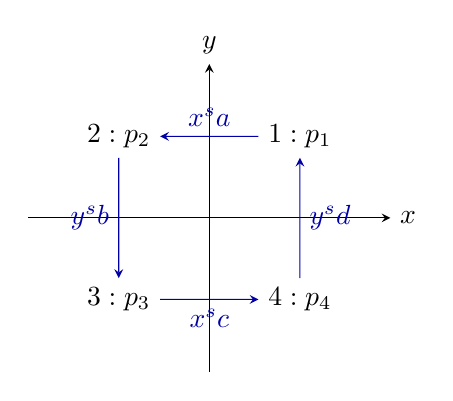
\begin{tikzpicture}[scale=1.15,>=stealth]
\draw[->] (-2,0)--(2,0) node[right] {\(x\)};
\draw[->] (0,-1.7)--(0,1.7) node[above] {\(y\)};
\node (q1) at (1,0.9) {\(1:p_1\)};
\node (q2) at (-1,0.9) {\(2:p_2\)};
\node (q3) at (-1,-0.9) {\(3:p_3\)};
\node (q4) at (1,-0.9) {\(4:p_4\)};
\draw[->,blue!65!black] (q1)--(q2) node[midway,above] {\(x^sa\)};
\draw[->,blue!65!black] (q2)--(q3) node[midway,left] {\(y^sb\)};
\draw[->,blue!65!black] (q3)--(q4) node[midway,below] {\(x^sc\)};
\draw[->,blue!65!black] (q4)--(q1) node[midway,right] {\(y^sd\)};
\end{tikzpicture}
\end{center}
相加得到环行相容条件
\[
x^s(a+c)+y^s(b+d)=0.
\]
这一条件也充分：给定 \(p_1,a,b,c,d\) 后，沿前三条边依次定义 \(p_2,p_3,p_4\)，相容等式恰好保证最后一条边的等式成立。因此没有遗漏其他环行条件。又因 \(x^s,y^s\) 互素，全部关系为
\[
a+c=y^s h,\qquad b+d=-x^s h\qquad(h\in S).
\]
证明也很直接：\(x^s\mid y^s(b+d)\) 推出 \(x^s\mid b+d\)，写 \(b+d=-x^sh\) 后再约去 \(x^s\)。这正是两生成元 \((x^s,y^s)\) 的合冲计算。

\ProseParagraphBreak
取 \(p=p_1\)，依次回代得到全部解
\[
\begin{aligned}
(p_1,p_2,p_3,p_4)
={}&p(1,1,1,1)+a(0,x^s,x^s,0)\\
&+b(0,0,y^s,y^s)+h(0,0,0,x^sy^s).
\end{aligned}
\]
这四个向量的系数唯一：先读第一坐标求 \(p\)，再由第二、第三、第四坐标顺次求 \(a,b,h\)。所以边条件解模是自由分次模
\[
S\oplus S(-s)^2\oplus S(-2s).
\]
四个自由生成元的内次数分别为 \(0,s,s,2s\)，所以这也是前面次数平移自由模的具体应用。其非零区域可以直接对照下面的图；灰色表示该生成元可能非零的象限，坐标轴上的值由相邻多项式一致决定。
\begin{center}
\begin{tikzpicture}[scale=0.75]
\begin{scope}[shift={(0,0)}]
\fill[gray!25] (-1,-1) rectangle (1,1);
\draw (-1.2,0)--(1.2,0);\draw (0,-1.2)--(0,1.2);
\node[below] at (0,-1.3) {\((1,1,1,1)\)};
\end{scope}
\begin{scope}[shift={(3.5,0)}]
\fill[gray!25] (-1,-1) rectangle (0,1);
\draw (-1.2,0)--(1.2,0);\draw (0,-1.2)--(0,1.2);
\node[below] at (0,-1.3) {左半平面：\(x^s\)};
\end{scope}
\begin{scope}[shift={(7,0)}]
\fill[gray!25] (-1,-1) rectangle (1,0);
\draw (-1.2,0)--(1.2,0);\draw (0,-1.2)--(0,1.2);
\node[below] at (0,-1.3) {下半平面：\(y^s\)};
\end{scope}
\begin{scope}[shift={(10.5,0)}]
\fill[gray!25] (0,-1) rectangle (1,0);
\draw (-1.2,0)--(1.2,0);\draw (0,-1.2)--(0,1.2);
\node[below] at (0,-1.3) {右下：\(x^sy^s\)};
\end{scope}
\end{tikzpicture}
\end{center}
前三个生成元只改变全平面或一侧半平面；第四个在右下象限同时含两个边界方程的幂，因而可以只修正这个角部，又不破坏两条邻边上的 \(C^r\) 条件。其系数 \(h\) 不由前三片决定，正是独立的角部修正。

\ProseParagraphBreak
四个生成元确实在原点也是 \(C^r\) 的。第二个对应左半平面上的 \(x^s\)、右半平面上的零，第三个对应下半平面上的 \(y^s\)、上半平面上的零；第四个是右半平面取 \(x^s\)、左半平面取零的函数，与下半平面取 \(y^s\)、上半平面取零的函数的乘积。每个一元分片函数的前 \(r=s-1\) 阶导数都在零处连续，乘以全局多项式及有限相加保持 \(C^r\)。因此上述全部解恰为整个平面的样条，顶点处没有遗漏的条件。

\ProseParagraphBreak
记 \(N(j)=\binom{j+2}{2}\) 当 \(j\ge0\)，而 \(N(j)=0\) 当 \(j<0\)。它是二元全次数不超过 \(j\) 的多项式空间维数。上述唯一表示逐项保持次数，故
\[
\dim_{\mathbb R}C_d^r(\Delta)=N(d)+2N(d-s)+N(d-2s).
\]
例如连续分片二次多项式对应 \(r=0,d=2\)，维数为 \(6+2\cdot3+1=13\)；若要求一阶光滑，则 \(r=1\)，维数变为 \(6+2=8\)。环行条件中的辅助元 \(h\) 正是四条边约束之间的关系所留下的自由量。这说明为什么实际维数不能只用四片的系数总数减去表面上列出的方程数。


\begin{chaptersummary}
自由消解逐层记录生成元之间的关系。分次极小性使微分在剩余域上变为零，因而各层各次的自由秩恰为 Tor 的分次维数。Hilbert 合冲定理进一步说明，在 \(n\) 个变量的多项式环上，有限生成分次模的极小自由消解不会超过 \(n\) 层。

\ProseParagraphBreak
计算时，模项序与 Schreyer 构造给出全部核关系，单位微分项则指出可以删去的可缩部分。正确的记录既要有微分相乘为零的等式，也要有像等于核的依据。Hilbert 级数能由各层次数的交错和恢复，但无法反过来决定 Betti 表；初始理想的单项式计数也必须与原理想的消解信息分开。样条实例把光滑拼接化为整除关系，进一步说明核、合冲模和次数计数怎样共同回答一个具体问题。
\end{chaptersummary}

\BookExercises
除题目另作说明外，多项式环均取标准分次。

\begin{exercise}\label{b3:ex:21-common-factor}
设 \(k\) 为域，在 \(S=k[x,y]\) 中令 \(I=(x^2,xy^2)\)。求 \(I\) 的全部关系，写出 \(S/I\) 的极小自由消解、分次 Betti 数与 Hilbert 级数。
\end{exercise}
\begin{solution}
若 \(ax^2+bxy^2=0\)，约去 \(x\) 得 \(ax+by^2=0\)。因 \(x,y\) 互素，\(b=-cx\)、\(a=cy^2\)。故消解为
\[
0\rightarrow S(-4)\xrightarrow{\binom{y^2}{-x}}S(-2)\oplus S(-3)
\xrightarrow{(x^2\ xy^2)}S\rightarrow S/I\rightarrow0.
\]
左映射单射，其余正合性由上述全部关系计算得出；各微分项在 \((x,y)\) 中，故极小。非零 Betti 数为 \(\beta_{0,0}=\beta_{1,2}=\beta_{1,3}=\beta_{2,4}=1\)，级数为 \((1-t^2-t^3+t^4)/(1-t)^2\)。标准单项式 \(y^a\ (a\ge0)\)、\(x\)、\(xy\) 也给出 \(1/(1-t)+t+t^2\)。
\end{solution}

\begin{exercise}\label{b3:ex:21-nakayama-bound}
设 \(k\) 为域，取 \(S=k[x]\)、\(M=k[x,x^{-1}]/k[x]\)，以通常次数分次。写出 \(M\) 的齐次 \(k\) 基，证明 \(M=xM\ne0\) 而 \(M_x=0\)，并说明分次 Nakayama 引理为何不适用。
\end{exercise}
\begin{solution}
齐次基为 \(\overline{x^{-r}}\ (r\ge1)\)，基向量的次数为 \(-r\)，故 \(M\ne0\) 且非零次数没有下界。又 \(\overline{x^{-r}}=x\overline{x^{-(r+1)}}\)，所以 \(M=xM\)。每个元素只涉及有限个负指数，乘足够大的 \(x\) 次幂后就落入 \(k[x]\)，在商中为零；因此局部化 \(M_x\) 为零。有限组生成元有共同最低次数，乘非负次数多项式不能生成更低次数，故 \(M\) 也非有限生成。\Cref{b3:lem:graded-nakayama}所需的次数下界在这里缺失。
\end{solution}

\begin{exercise}\label{b3:ex:21-direct-sum-shifts}
设 \(k\) 为域，\(S=k[x,y]\)，求 \(M=S/(x^2)\oplus (S/(y))(-1)\) 的极小自由消解与分次 Betti 数。
\end{exercise}
\begin{solution}
两部分分别由乘 \(x^2\) 与乘 \(y\) 的单射消解，直和后为
\[
0\rightarrow S(-2)^2\xrightarrow{\left(\begin{smallmatrix}x^2&0\\0&y\end{smallmatrix}\right)}
S\oplus S(-1)\rightarrow M\rightarrow0.
\]
第二行目标基次数一，故第二列的 \(y\) 仍使总次数为二。矩阵项都在极大齐次理想中，因此 \(\beta_{0,0}=\beta_{0,1}=1\)、\(\beta_{1,2}=2\)。
\end{solution}

\begin{exercise}\label{b3:ex:21-detect-localization}
设 \(k\) 为域，\(S=k[x_1,\ldots,x_n]\)、\(\mathfrak m=(x_1,\ldots,x_n)\)，\(M\) 为有限生成分次 \(S\) 模。证明 \(M_{\mathfrak m}=0\) 当且仅当 \(M=0\)。进一步说明分次极小消解局部化于 \(\mathfrak m\) 后仍极小。
\end{exercise}
\begin{solution}
若 \(M_{\mathfrak m}=0\)，取有限组生成元并合并各自使其为零的分母，得 \(s\notin\mathfrak m\) 且 \(sM=0\)。写 \(s=c+s_+\)、\(c\in k^\times\)，模 \(\mathfrak m\) 得 \(c(M/\mathfrak mM)=0\)，故商为零，再由\cref{b3:lem:graded-nakayama}得 \(M=0\)。反向直接成立。局部化保持正合与自由，极小微分的系数仍落入 \(\mathfrak mS_{\mathfrak m}\)，所以得到局部极小消解，且非零自由项不会消失。
\end{solution}

\begin{exercise}\label{b3:ex:21-projective-graded-free}
设 \(k\) 为域，\(S=k[x,y]\)，\(F=S(-2)\oplus S\)，记两个齐次基向量为 \(e_1,e_2\)，其内次数分别为二、零。考虑矩阵
\[
E=\begin{pmatrix}1&0\\xy&0\end{pmatrix}.
\]
验证它定义一个保持次数的幂等自同态，求 \(P=\operatorname{im}E\)、\(Q=\ker E\) 的齐次自由基和次数平移，并写出 \(F=P\oplus Q\) 的分次分解。
\end{exercise}
\begin{solution}
有 \(E(e_1)=e_1+xy e_2\)、\(E(e_2)=0\)，两者分别为次数二的齐次向量和零向量，所以 \(E\) 保持次数；直接计算得 \(E^2=E\)。其像以 \(e_1+xy e_2\) 为齐次自由基，次数二，故 \(P\cong S(-2)\)；核以 \(e_2\) 为齐次自由基，次数零，故 \(Q\cong S\)。分解由
\[
a e_1+b e_2=a(e_1+xy e_2)+(b-a xy)e_2
\]
给出，两个分量的交为零。对齐次向量，右边两项仍具有相同的总内次数，所以这是分次直和分解。它具体实现了\cref{b3:prop:graded-projective-free}中的齐次自由性，不能仅按矩阵系数的次数忽略目标基的次数平移。
\end{solution}

\begin{exercise}\label{b3:ex:21-polynomial-sequence-point}
设 \(k\) 为域，把\cref{b3:lem:polynomial-module-sequence}用于 \(A=k\)、\(B=k[t]\)、\(M=k\)，其中 \(t\) 作用为乘 \(\lambda\in k\)。写出对应短正合列，并由它计算 \(\operatorname{Tor}_1^B(M,M)\)。
\end{exercise}
\begin{solution}
两份 \(B\otimes_kM\) 都同构于 \(B\)，\(\delta\) 成为乘 \(t-\lambda\)，而 \(\varepsilon\) 是在 \(\lambda\) 处求值。因此得到 \(0\rightarrow B\xrightarrow{t-\lambda}B\rightarrow M\rightarrow0\)。张量 \(M\) 后微分为零，故 \(\operatorname{Tor}_1^B(M,M)\simeq M\)。当 \(\lambda\ne0\) 时该例按通常分次并非分次模例子，但引理本来适用于任意模。
\end{solution}

\begin{exercise}\label{b3:ex:21-infinite-singular-resolution}
设 \(k\) 为域，\(R=k[\varepsilon]/(\varepsilon^2)\)。证明 \(k=R/(\varepsilon)\) 有无限极小自由消解，计算全部 \(\operatorname{Tor}_i^R(k,k)\)，并指出 Hilbert 合冲定理不能直接用于此环的原因。
\end{exercise}
\begin{solution}
乘 \(\varepsilon\) 的核与像均为 \(k\varepsilon\)，所以
\(\cdots\xrightarrow{\varepsilon}R\xrightarrow{\varepsilon}R\rightarrow k\rightarrow0\)
正合。局部极大理想为 \((\varepsilon)\)，因此消解极小，张量 \(k\) 后全为零微分，得每个 \(i\ge0\) 的 Tor 均为 \(k\)。所以投射维数无限。\(R\) 是多项式环的商而非域上的多项式环；商去非零理想不保持上述整体维数上界。
\end{solution}

\begin{exercise}\label{b3:ex:21-cubic-powers}
设 \(k\) 为域，在 \(S=k[x,y,z]\) 中写出 \(S/(x^2,y^2,z^2)\) 的极小消解各项、分次 Betti 数和 Hilbert 级数，不必把所有微分展开成矩阵。
\end{exercise}
\begin{solution}
逐次商后每个新变量的平方仍是非零因子：商可按其余变量的单项式写成关于该变量的多项式，乘其平方只是平移指数。因此用 Koszul 消解得
\(F_0=S\)、\(F_1=S(-2)^3\)、\(F_2=S(-4)^3\)、\(F_3=S(-6)\)。微分系数为变量平方，故极小，\(\beta_{i,2i}=\binom3i\)。级数为 \((1-t^2)^3/(1-t)^3=(1+t)^3\)，总维数八，也由各变量指数为零或一的八个单项式得到。
\end{solution}

\begin{exercise}\label{b3:ex:21-cancel-hilbert-not-exact}
设 \(k\) 为域，\(S=k[x]\) 取标准分次，\(M=S/(x)\)。考虑保持次数的增广列
\[
0\longrightarrow S(-1)\oplus S\xrightarrow{\mathrm{d}}S^2
\xrightarrow{\varepsilon}M\longrightarrow0,
\]
其中 \(\mathrm{d}(a,b)=(xa,0)\)、\(\varepsilon(c,d)=c\bmod x\)。验证 \(\varepsilon\mathrm{d}=0\)，比较自由项的 Hilbert 交错和与 \(H_M(t)\)，并计算 \(\ker\mathrm{d}\) 及 \(\ker\varepsilon/\operatorname{im}\mathrm{d}\)，判断它是否为 \(M\) 的自由消解。
\end{exercise}
\begin{solution}
由 \(xa\bmod x=0\)，有 \(\varepsilon\mathrm{d}=0\)，且 \(\varepsilon\) 满射。自由项的交错和为
\[
\frac{2}{1-t}-\frac{t+1}{1-t}=1=H_M(t).
\]
然而，整环性给出 \(\ker\mathrm{d}=0\oplus S\cong S\)。又
\(\ker\varepsilon=xS\oplus S\)、\(\operatorname{im}\mathrm{d}=xS\oplus0\)，所以 \(\ker\varepsilon/\operatorname{im}\mathrm{d}\cong S\)。两处都不正合，故这不是消解。两个多出的非零模具有相同 Hilbert 级数，恰好在交错和中抵消；与\cref{b3:exm:hilbert-euler-not-exact}一样，Euler 计数不能代替核与像的检验。
\end{solution}

\begin{exercise}\label{b3:ex:21-rank-euler}
设 \(k\) 为域，\(n\ge1\)，\(S=k[x_1,\ldots,x_n]\) 取标准分次，\(M\ne0\) 为有限生成分次挠 \(S\) 模。记 \(B(M)=\sum_{i=0}^n\beta_i(M)\)。证明 \(B(M)\ge2\)，且等号成立当且仅当存在整数 \(a\) 和非零的正次数齐次多项式 \(f\in S\)，使 \(M\cong(S/(f))(-a)\)。
\end{exercise}
\begin{solution}
置 \(\mathfrak m=(x_1,\ldots,x_n)\)。Hilbert 合冲定理使极小消解在第 \(n\) 层以后为零，所以 \(B(M)\) 是全部 Betti 数的有限总和。\(M\ne0\) 给出 \(\beta_0\ge1\)。若 \(\beta_1=0\)，则 \(F_1=0\)，正合性使 \(F_0\cong M\)，与非零自由模不能为挠模矛盾；因此 \(\beta_1\ge1\)，遂有 \(B(M)\ge2\)。

若等号成立，则 \(\beta_0=\beta_1=1\)，其余 Betti 数全为零。极小消解因此为
\[
0\longrightarrow S(-b)\xrightarrow{f}S(-a)
\longrightarrow M\longrightarrow0.
\]
左映射单射使 \(f\ne0\)，保持次数使 \(f\) 齐次且次数为 \(b-a\)，极小性又使 \(f\in\mathfrak m\)，故 \(b-a>0\)。余核就是 \((S/(f))(-a)\)。反之，对这样的 \(f\)，乘 \(f\) 在整环上单射，所给两项消解极小，所以总 Betti 数为二。这个结论也符合\cref{b3:prop:betti-rank-euler}中的 \(\beta_0-\beta_1=0\)。
\end{solution}

\begin{exercise}\label{b3:ex:21-mixed-shifts}
设 \(k\) 为域，在 \(S=k[x,y]\) 中考虑行矩阵 \((x^2\ y)\)。确定使其保持次数的自由项，求其核以及余核 \(S/(x^2,y)\) 的极小消解，并检验每个矩阵项的次数。
\end{exercise}
\begin{solution}
源为 \(S(-2)\oplus S(-1)\)，目标为 \(S\)。由互素性，全部关系由 \((-y,x^2)\) 生成，其总次数是三，所以左项为 \(S(-3)\)。第一列系数 \(-y\) 的次数为 \(3-2=1\)，第二列系数 \(x^2\) 的次数为 \(3-1=2\)。得到 \(S/(x^2,y)\) 的长度二极小消解，首映射因整环性单射。
\end{solution}

\begin{exercise}\label{b3:ex:21-different-components}
设 \(k\) 为域，\(F=k[x,y]e_1\oplus k[x,y]e_2\)，取位置优先且 \(e_1\succ e_2\) 的模项序。证明 \(g_1=xe_1+e_2\)、\(g_2=ye_2\) 是其生成子模的 Gröbner 基，并求全部合冲关系。
\end{exercise}
\begin{solution}
两首项位置不同，不存在需检验的 \(S\)-向量，故由\cref{b3:prop:module-groebner-algorithm}为 Gröbner 基。也可直接看：若 \(a\ne0\)，\(ag_1+bg_2\) 的第一分量为 \(ax\ne0\)，首项被 \(xe_1\) 整除；若 \(a=0\)，非零首项被 \(ye_2\) 整除。若总和为零，第一分量给出 \(a=0\)，第二分量再得 \(b=0\)，所以合冲模为零。
\end{solution}

\begin{exercise}\label{b3:ex:21-same-component}
设 \(k\) 为域，\(F=k[x,y]e_1\oplus k[x,y]e_2\)，\(G=(x^2e_1,ye_1,e_2)\)。计算其 Schreyer 关系，并求 \(F/(G)\)。
\end{exercise}
\begin{solution}
只有前两个首项位置相同，得到关系 \(y\epsilon_1-x^2\epsilon_2\)。第三位置无法与其余项抵消，所以它生成全部合冲模。商中 \(e_2=0\)，第一分量模掉 \((x^2,y)\)，故 \(F/(G)\simeq k[x]/(x^2)\)。要讨论分次消解，可给三个源生成元分别赋次数二、一、零，关系次数为三。
\end{solution}

\begin{exercise}\label{b3:ex:21-redundant-original-generators}
设 \(k\) 为域，\(S=k[x,y,z]\)，令 \(F=(x\ y\ z\ x+y+z)\)、\(G=(x\ y\ z)\)。取
\[
U=\begin{pmatrix}1&0&0\\0&1&0\\0&0&1\\0&0&0\end{pmatrix},
\qquad
V=\begin{pmatrix}1&0&0&1\\0&1&0&1\\0&0&1&1\end{pmatrix}.
\]
先求一个列生成 \(\ker G\) 的矩阵 \(T\)，再利用 \(UT\) 与 \(I_4-UV\) 构造 \(\ker F\) 的全部生成元，写出这些生成元之间的关系，并指出常数关系怎样使消解极小化为变量 \(x,y,z\) 的 Koszul 消解。
\end{exercise}
\begin{solution}
有 \(G=FU\)、\(F=GV\)。变量 \(x,y,z\) 构成正则序列，所以 \(G\) 的核由三列 Koszul 关系生成，记其矩阵为 \(T\)。\Cref{b3:prop:kernel-generator-change}给出 \(\ker F\) 的生成元
\[
\begin{gathered}
s_{12}=(-y,x,0,0),\qquad s_{13}=(-z,0,x,0),\\
s_{23}=(0,-z,y,0),\qquad c=(-1,-1,-1,1).
\end{gathered}
\]
前三列来自 \(UT\)，最后一列是 \(I_4-UV\) 的唯一非零列。若它们的线性组合为零，第四坐标先使 \(c\) 的系数为零；剩下前三列的全部关系由 Koszul 复形的下一层给出，即
\[
z s_{12}-y s_{13}+x s_{23}=0.
\]
关系 \(c\) 表示第四生成元等于前三个之和，其非零常数系数消去一个同为次数一的源、目标基向量。留下的理想生成组为 \((x,y,z)\)，再接上 \(S\to S/(x,y,z)\)，便得到长度三的极小 Koszul 消解。若以理想 \((x,y,z)\) 为末项，则相应消解长二。
\end{solution}

\begin{exercise}\label{b3:ex:21-divisibility-relations}
设 \(k\) 为域，给 \(S=k[x,y]\) 中的三个单项式 \(x^3,x^2y,xy^2\) 求最小关系生成组，并求商环 \(S/(x^3,x^2y,xy^2)\) 的 Hilbert 级数。
\end{exercise}
\begin{solution}
三个生成元都含公共因子 \(x\)，在整环中约去它，关系与 \(x^2,xy,y^2\) 相同，故由 \((y,-x,0)\)、\((0,y,-x)\) 自由生成。所得极小消解各项为 \(S\)、\(S(-3)^3\)、\(S(-4)^2\)，级数为 \((1-3t^3+2t^4)/(1-t)^2\)。约去公共因子不改变关系系数，却改变生成元和关系的内次数。
\end{solution}

\begin{exercise}\label{b3:ex:21-unit-homotopy}
设 \(k\) 为域，\(S=k[x_1,\ldots,x_n]\) 取标准分次，\(a\in\mathbb Z\)、\(c\in k^\times\)。对两项复形 \(0\rightarrow S(-a)\xrightarrow{c}S(-a)\rightarrow0\)，写出恒等映射与零映射之间的链同伦。解释为什么它可以从消解中删去。
\end{exercise}
\begin{solution}
令从低次项到高次项的同伦映射为乘 \(c^{-1}\)，其余同伦分量为零。则两项上分别有 \(\mathrm{d}h=1\)、\(h\mathrm{d}=1\)，故 \(\mathrm{d}h+h\mathrm{d}\) 为恒等。这个复形可缩，特别正合；若它是某消解的直和项，去掉后各同调不变。仅在微分矩阵里看见一个非零常数还须先作相容换基，才能保证它确实构成直和项。
\end{solution}

\begin{exercise}\label{b3:ex:21-tor-socle}
设 \(k\) 为域，\(A=k[x,y]/(x^2,y^3)\)。直接用以 \(A\) 为系数的两元 Koszul 复形求 \(\operatorname{Tor}_2^{k[x,y]}(A,k)\) 的维数与内次数。
\end{exercise}
\begin{solution}
最高同调对应被 \(x,y\) 同时零化的元素。把元素按基 \(1,x,y,xy,y^2,xy^2\) 展开，乘 \(x\) 为零使只剩 \(x,xy,xy^2\) 的组合，再乘 \(y\) 为零只剩 \(kxy^2\)。此元素内次数三，加上 \(e_x\wedge e_y\) 的次数二，所得 Tor 为一维且内次数五，符合完整消解左项 \(S(-5)\)。
\end{solution}

\begin{exercise}\label{b3:ex:21-betti-specialization}
设 \(k\) 为域，\(a\in k\)，在 \(S=k[x,y]\) 中令 \(I_a=(x^2,xy+ay^2,y^3)\)。证明所有 \(S/I_a\) 的 Hilbert 级数相同，但 \(a=0\) 与 \(a\ne0\) 的 Betti 表不同。
\end{exercise}
\begin{solution}
字典序 \(x\succ y\) 下这三个多项式构成 Gröbner 基：前两者的 \(S\)-多项式先约化成 \(a^2y^3\)，第二、第三对约化为 \(ay^4\)，均由 \(y^3\) 消去；第一、第三对首项互素。标准单项式恒为 \(1,x,y,y^2\)，级数为 \(1+2t+t^2\)。

若 \(a\ne0\)，恒等式
\(yx^2-(x-ay)(xy+ay^2)=a^2y^3\)
使第三生成元冗余；前两者互素，构成二次正则序列，非零 Betti 多项式为 \(1,2t^2,t^4\)。若 \(a=0\)，则为正文的 \((x^2,xy,y^3)\)，Betti 多项式为 \(1,2t^2+t^3,t^3+t^4\)。消去三次生成元的系数涉及 \(a^{-2}\)，因此不能把一般参数下的极小化直接代入 \(a=0\)。
\end{solution}

\begin{exercise}\label{b3:ex:21-kernel-certificate}
设 \(k\) 为域，\(S=k[x,y,z]\)、\(F=(x^2\ xy\ xz)\)。有人以
\[
K=\begin{pmatrix}-y&-z\\x&0\\0&x\end{pmatrix}
\]
作为 \(\ker F\) 的生成矩阵。验证 \(FK=0\)，证明它遗漏了关系 \((0,-z,y)\)，补全核的生成组，并写出这些生成元的全部关系。
\end{exercise}
\begin{solution}
直接相乘得 \(FK=0\)，且 \(s_{23}=(0,-z,y)\) 也被 \(F\) 零化。但 \(K\) 的像中每个向量的第二、第三坐标都可被 \(x\) 整除；\(s_{23}\) 的这两坐标不能如此，故它不属于 \(\operatorname{im}K\)。等价地，模掉 \(x\) 后，\(K\) 的像只可能有第一坐标，而 \(s_{23}\) 的后两坐标非零。

在整环中约去 \(F=x(x\ y\ z)\) 的公共因子 \(x\)，得到 \(\ker F=\ker(x\ y\ z)\)。变量 Koszul 复形遂给出全部核生成元
\(s_{12}=(-y,x,0)\)、\(s_{13}=(-z,0,x)\)、\(s_{23}=(0,-z,y)\)，而它们的关系模由 \((z,-y,x)\) 生成，即 \(z s_{12}-y s_{13}+x s_{23}=0\)。所以微分相乘为零只证明给出的列是关系，不能证明全部关系已经找齐。
\end{solution}

\begin{exercise}\label{b3:ex:21-top-degree-bound}
设 \(k\) 为域，\(S=k[x_1,\ldots,x_n]\) 取标准分次，\(M\ne0\) 为有限生成分次 \(S\) 模，\(b\in\mathbb Z\)。若 \(M_j=0\) 对所有 \(j>b\) 成立，证明 \(\beta_{i,j}(M)=0\) 当 \(j>b+i\)。
\end{exercise}
\begin{solution}
以 \(M\) 为系数的变量 Koszul 复形第 \(i\) 项是 \(M(-i)^{\binom ni}\)，其次数 \(j\) 部分为若干 \(M_{j-i}\) 的直和。当 \(j>b+i\) 时该项为零，同调对应次数也为零；再由 Tor 与 Betti 数的等式得到结论。该上界来自各项本身为零，不需要预先求出微分的秩。
\end{solution}


\begin{exercise}\label{b3:ex:21-polynomial-inhomogeneous}
设 \(k\) 为域，在 \(S=k[x,y]\) 上求 \(x^2u+xyv=x^3\) 的全部多项式解，并说明把右端改为 \(x\) 时为何无解。
\end{exercise}
\begin{solution}
整环中约去 \(x\)，得到 \(xu+yv=x^2\)。特解为 \((x,0)\)，核由 \((y,-x)\) 生成，故全部解为 \(u=x+yh,v=-xh\)，\(h\in S\)。右端为 \(x\) 时约去 \(x\) 得 \(xu+yv=1\)，在原点求值即矛盾。若工作环改为 \(S_x\)，则 \((u,v)=(x^{-1},0)\) 是后一方程的解；这再次说明解集依赖工作环。
\end{solution}

\begin{optionalexercise}\label{b3:ex:21-spline-strips}
用直线 \(x=0\) 与 \(x=1\) 将 \(\mathbb R^2\) 分成三条闭区域，每片取 \(\mathbb R[x,y]\) 中的多项式，要求它们作 \(C^r\) 拼接，\(r\ge0\)。求全部解的唯一参数表示，以及每片全次数不超过整数 \(d\ge0\) 时的实向量空间维数。
\end{optionalexercise}
\begin{solution}
置 \(s=r+1\)，按从左到右排列分片。由\cref{b3:prop:spline-divisibility}，全部解唯一写成
\[
(p_1,p_2,p_3)=\bigl(p,\ p+x^sa,\ p+x^sa+(x-1)^sb\bigr),
\qquad p,a,b\in\mathbb R[x,y].
\]
两条直线不相交，因此没有内部顶点的额外拼接问题。若三个分片次数均不超过 \(d\)，由逐次作差可知 \(\deg p\le d\)、\(\deg a,\deg b\le d-s\)；反向这些限制显然足够。于是维数为 \(N(d)+2N(d-s)\)，其中 \(N(j)=\binom{j+2}{2}\) 对 \(j\ge0\)，负指标时为零。这里关系含常数，使用的是次数滤过；不能未经说明就把 \((x-1)^s\) 当成齐次元。
\end{solution}
